% This is based on "sig-alternate.tex" V1.9 April 2009
% This file should be compiled with V2.4 of "sig-alternate.cls" April 2009
%
% ---------------------------------------------------------------------------------------------------------------
% This .tex source uses a .bib file (from which the .bbl file % is produced).
% REMEMBER HOWEVER: After having produced the .bbl file, and prior to final
% submission, you *NEED* to 'insert' your .bbl file into your source .tex file
% so as to provide ONE 'self-contained' source file.

\documentclass[11pt,twocolumn]{article}
\usepackage[11pt,nocopyright]{sigmin}
\usepackage[square,comma,numbers,sort&compress]{natbib}
\usepackage{times}
\usepackage{microtype}
\usepackage{color}
\usepackage{graphicx}
\usepackage{listings}
\usepackage{multirow}
\usepackage{url}
\lstset{
  numbers=left, frame=lines, tabsize=2, captionpos=b, numberstyle=\tiny,
  columns=fullflexible, showstringspaces=false, basicstyle=\footnotesize\ttfamily,
  extendedchars=true, breaklines=true
}

\setlength{\columnsep}{.25in}

\begin{document}
\title{Intel SGX Explained}
\author{Victor Costan, Staphany Park, and Srinivas Devadas \\ \em MIT CSAIL}
\date{}

\maketitle

\begin{abstract}

Intel's Software Guard Extensions (SGX) is a set of extensions to the Intel
architecture that aims to provide integrity and privacy guarantees to
security-sensitive computation performed on a computer where all the privileged
software (kernel, hypervisor, etc) is potentially malicious.

This paper analyzes Intel SGX, based on the 3
papers~\cite{mckeen2013sgx, anati2013sgx, hoekstra2013sgx} that introduced it,
on its reference manual~\cite{intel2014sgx2manual}, and on two patent
applications~\cite{intel2013patent1, intel2013patent2}. We use the papers and
reference manual as primary data sources, and only draw on the patents to fill
in missing information.

We explain the threat model and mechanisms used by SGX and analyze their
security properties. In conclusion, we agree with the Intel authors that SGX
protects the integrity of sensitive computation, and provides some privacy
guarantees. We show straight-forward methods for obtaining the memory access
patterns in an SGX program. We argue that memory access pattern leaks can allow
an adversary to learn private information, and analyze the limitations of SGX
from this
perspective.

\end{abstract}

\section{Overview}
\label{sec:intro}

Secure remote computation (Figure~\ref{fig:remote_computation}) is the problem
of executing software on a remote computer \textbf{owned and maintained by an
untrusted party}, with some integrity and privacy guarantees. In the general
setting, secure remote computation is an unsolved problem. Fully Homomorphic
Encryption \cite{gentry2009fhe} solves the problem for a limited family of
computations, but has an unpractical performance overhead
\cite{naehrig2011can}.

\begin{figure}[hbt]
  \center{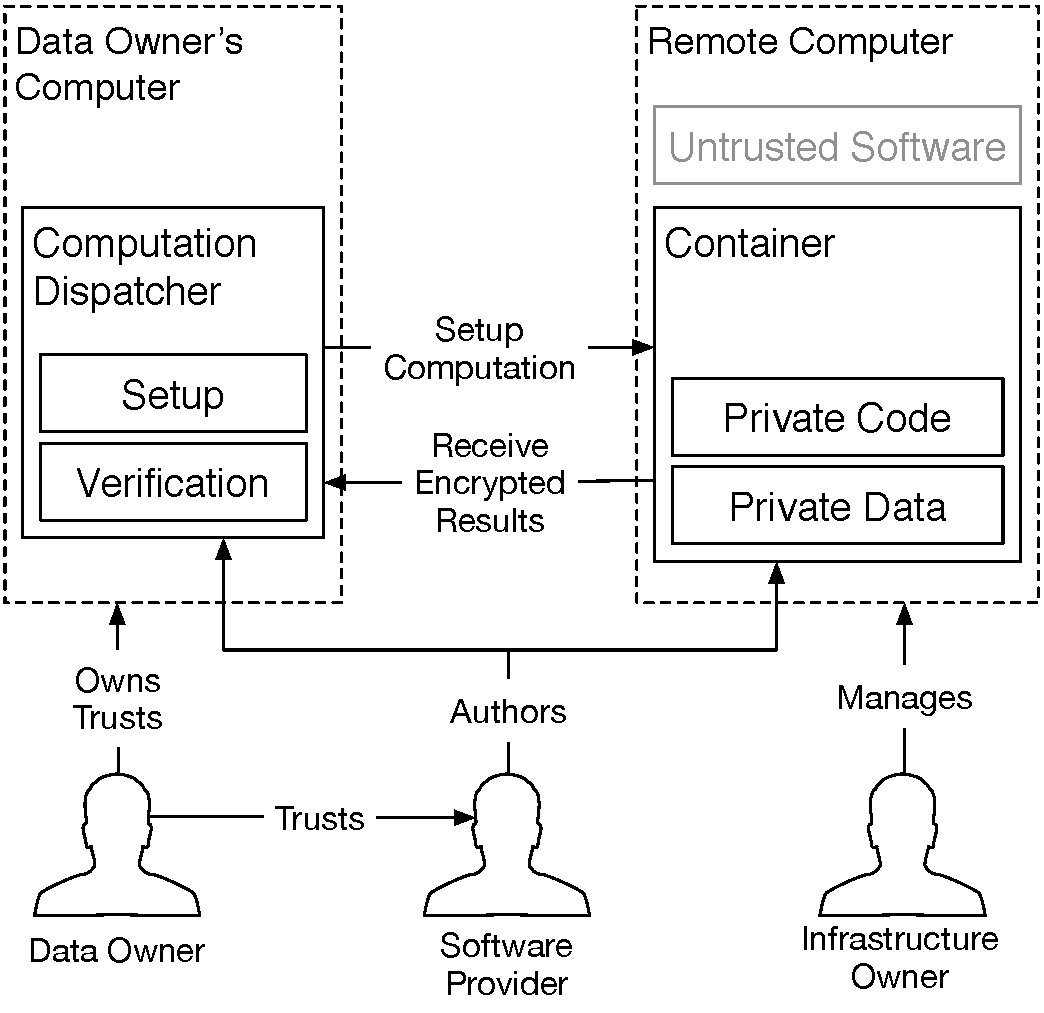
\includegraphics[width=75mm]{figures/remote_computation.pdf}}
  \caption{
    Secure remote computation. A user relies on a remote computer, owned by an
    untrusted party, to perform some computation on her data. The user has some
    assurance of the computation's integrity and privacy.
  }
  \label{fig:remote_computation}
\end{figure}

Intel's Software Guard Extensions (SGX) is the latest iteration in a long line
of trusted computing (Figure~\ref{fig:trusted_computing}) designs, which aim to
solve the secure remote computation problem by leveraging trusted hardware in
the remote computer. The trusted hardware establishes a secure container, and
the remote computation service user uploads the desired computation and data
into the secure container. The trusted hardware protects the data's privacy
and integrity while the computation is being performed on it.

\begin{figure}[hbt]
  \center{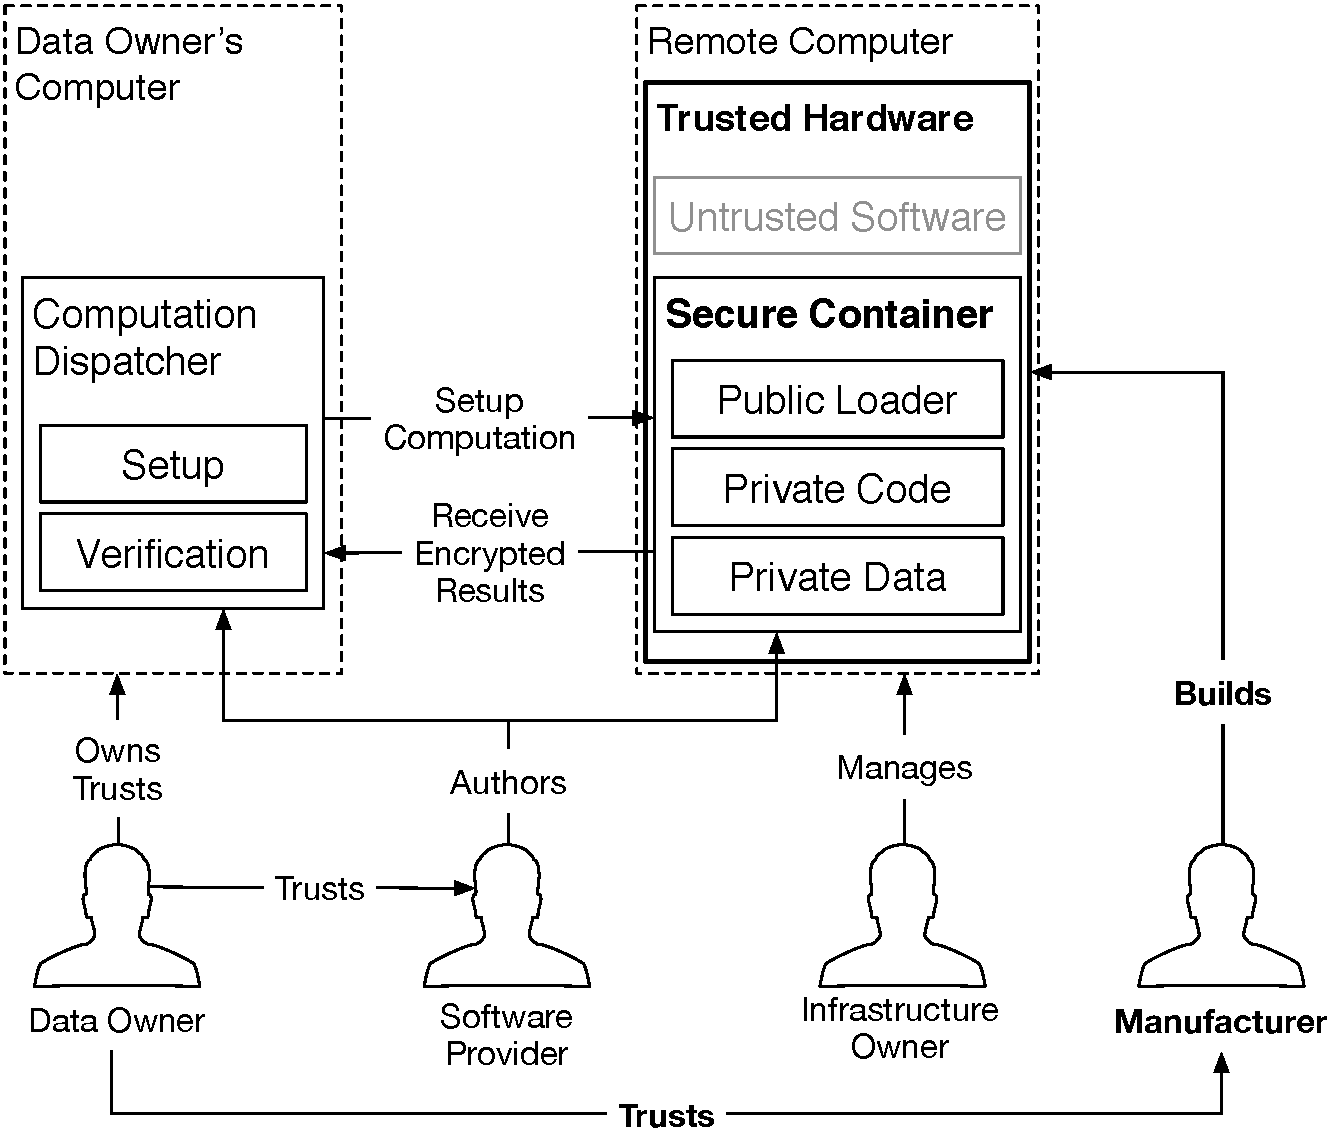
\includegraphics[width=85mm]{figures/trusted_computing.pdf}}
  \caption{
    Trusted computing. The user trusts the manufacturer of a piece of hardware
    in the remote computer, and entrusts her data to a secure container hosted
    by the secure hardware.
  }
  \label{fig:trusted_computing}
\end{figure}

SGX relies on \textit{software attestation}, like its predecessors, the
TPM~\cite{grawrock2003tpm} and TXT~\cite{grawrock2009txt}. Attestation
(Figure~\ref{fig:generic_attestation}) proves to a user that she is
communicating with a specific piece of software running in a secure container
hosted by the trusted hardware. The proof is a cryptographic signature that
certifies the hash of the secure container's contents. It follows that the
remote computer's owner can load any software in a secure container, but the
remote computation service user will refuse to load her data into a secure
container whose contents hash that does not match the expected value.

\begin{figure}[hbt]
  \center{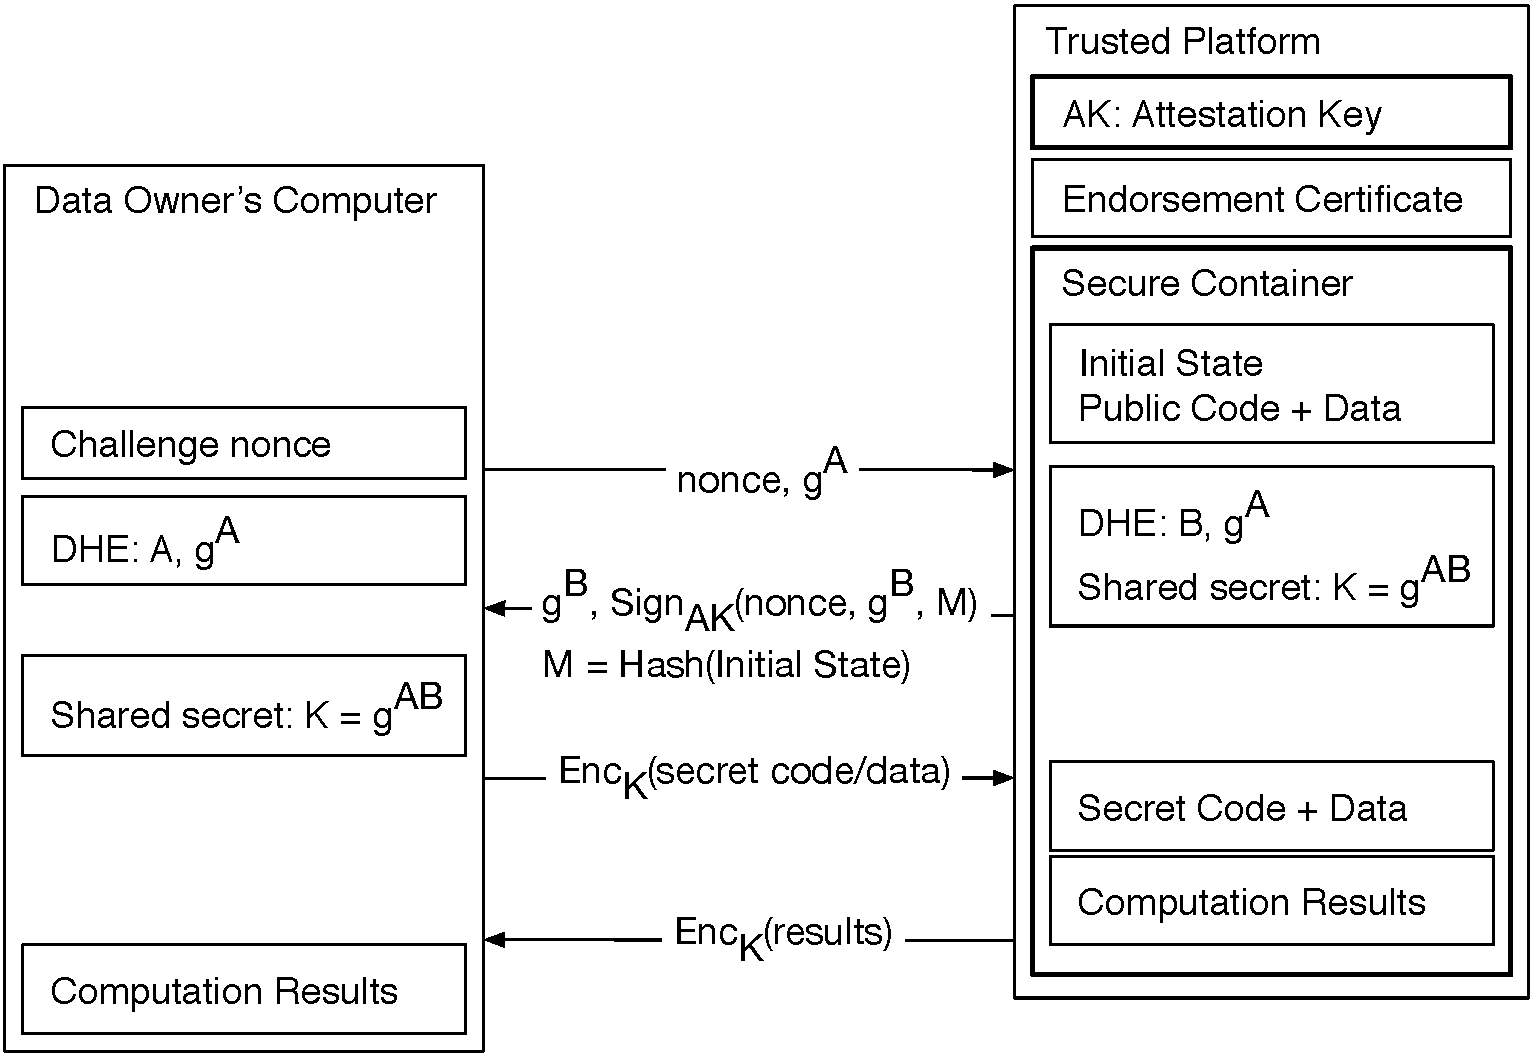
\includegraphics[width=85mm]{figures/generic_attestation.pdf}}
  \caption{
    Software attestation proves to a remote computer that it is communicating
    with a specific secure container hosted by a trusted platform. The proof is
    an attestation signature produced by the platform's secret attestation key.
    The signature covers the container's initial state, a challenge nonce
    produced by the remote computer, and a message produced by the container.
  }
  \label{fig:generic_attestation}
\end{figure}

The remote computation service user verifies the \textit{attestation key} used
to produce the signature against an \textit{endorsement certificate} created by
the trusted hardware's manufacturer. The certificate states that the
attestation key is only known to the trusted hardware, and only used for the
purpose of attestation.

SGX stands out from its predecessors by the amount of code covered by the
attestation, which is in the Trusted Computing Base (TCB) for the system using
hardware protection. The attestations produced by the original TPM design
covered all the software running on a computer, and TXT attestations covered
the code inside a VMX \cite{uhlig2005vmx} virtual machine. In SGX, an
\textit{enclave} (secure container) only contains the private data in a
computation, and the code that operates on it.

For example, a cloud service that performs image processing on confidential
medical images could be implemented by having users upload encrypted images.
The users would send the encryption keys to software running inside an enclave.
The enclave would contain the code for decrypting images, the image processing
algorithm, and the code for encrypting the results. The code that receives the
uploaded encrypted images and stores them would be left outside the enclave.

An SGX-enabled processor protects the integrity and privacy of the computation
inside an enclave by isolating the enclave's code and data from the outside
environment, including the operating system and hypervisor, and hardware
devices attached to the system bus. At the same time, the SGX model remains
compatible with the traditional software layering in the Intel architecture,
where the OS kernel and hypervisor manage the computer's resources.


\subsection{SGX Lightning Tour}
\label{sec:intro_sgx}

SGX sets aside a memory region, called the \textit{Processor Reserved Memory}
(PRM, \S~\ref{sec:prm}). The CPU protects the PRM from all non-enclave memory
accesses, including kernel, hypervisor and SMM (\S~\ref{sec:rings}) accesses,
and DMA accesses (\S~\ref{sec:motherboard}) from peripherals.

The PRM holds the \textit{Enclave Page Cache} (EPC, \S~\ref{sec:epc}), which
consists of 4KB pages that store enclave code and data. The system software,
which is untrusted, is in charge of assigning EPC pages to enclaves. The CPU
tracks each EPC page's state in the \textit{Enclave Page Cache Metadata} (EPCM,
\S~\ref{sec:epcm}), to ensure that each EPC page belongs to exactly one
enclave.

The initial code and data in an enclave is loaded by untrusted system software.
During the setup stage (\S~\ref{sec:lifecycle}), the system software asks the
CPU to copy data from unprotected memory (outside PRM) into EPC pages, and
assigns the pages to the enclave being setup (\S~\ref{sec:epcm}). This
means that the initial enclave state is known to the system software.

After all the enclave's pages are loaded into EPC, the system software asks the
CPU to mark the enclave as initialized, at which point application software can
run the code inside the enclave. After an enclave is initialized, the loading
method described above is disabled.

While an enclave is loaded, its contents is cryptographically hashed by the
CPU. When the enclave is initialized, the hash is finalized, and becomes the
enclave's \textit{measurement hash}.

A remote party can undergo an \textit{attestation} process to convince itself
that it is communicating with a specific enclave running in a secure
environment. The remote party generates a random challenge and sends it to the
enclave. After an intricate sequence of steps, the remote party receives an
\textit{attestation signature} that covers the challenge, the enclave's
measurement hash, and a message generated by the enclave. The attestation
signature is created by a secret CPU attestation key, which is covered by an
\textit{attestation certificate} rooted at Intel's manufacturer key.

Provided that the remote party trusts Intel's root key, attestation convinces
it that the message in the attestation was generated by a specific enclave
running in an SGX environment. If the message is a step in a Diffie-Hellman key
exchange, the remote party can be assured that the resulting symmetric key is
only shared between it and the attested enclave.

\section{Background}
\label{sec:background}

Arguing about the security of an application running on an mainstream computer
using the Intel architecture requires understanding the interactions between
all the parts of an x86 execution environment. This section provides an
overview of the features referenced by the rest of the paper. Unless specified
otherwise, the information in this section can be found in Intel's
\textit{Software Development Manual} \cite{intel2014sdm} (SDM).

Each of the sub-sections below explains how its information is relevant to
to SGX, but does not introduce any SGX concepts. Experienced readers can safely
skip this section and refer back if necessary.


\subsection{Software Privilege Levels}
\label{sec:rings}

In an Infrastructure-as-a-Service (IaaS) cloud environment, such as Amazon EC2,
commodity CPUs run software at four different privilege levels, illustrated in
Figure~\ref{fig:cpu_rings} and described below. The rest of the section
describes the privilege levels. We also point to successful exploits that
execute at each privilege level, motivating the SGX design decision to assume
that the host computer has malicious software running at all privilege levels.

\begin{figure}[hbtp]
  \center{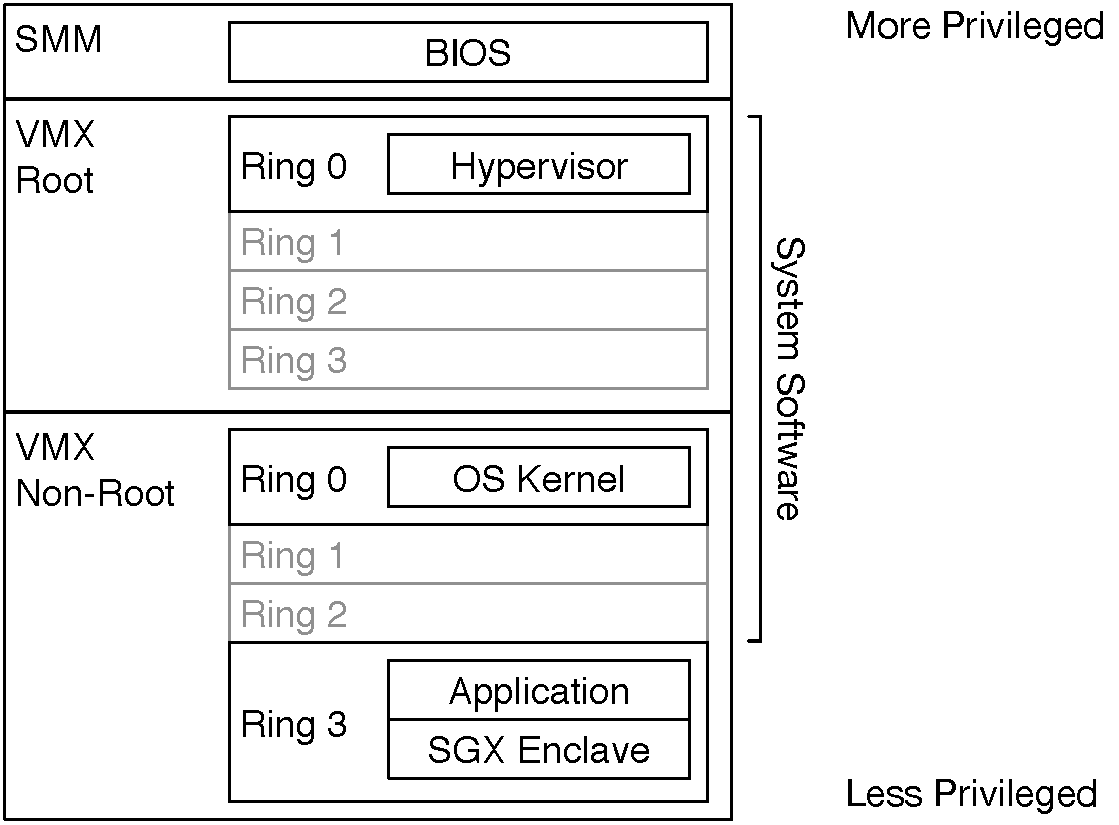
\includegraphics[width=50mm]{figures/cpu_rings.pdf}}
  \caption{
    The privilege levels in the x86 architecture, and the software that
    typically runs at each security level.
  }
  \label{fig:cpu_rings}
\end{figure}

\textit{System Management Mode} (SMM) is intended for use by the motherboard
manufacturers to implement features such as fan control and deep sleep, and/or
to emulate missing hardware. SMM mode is entered by asserting the SMI\# pin on
the CPU, which was initially designed exclusively for hardware use. However,
the southbridges on most motherboards provide a method for privileged
code\footnote{the hypervisor or operating system kernel} to get the SMI\# pin
asserted\footnote{Most southbridges assert \texttt{SMI\#} when a byte is
  written to port 0xb2 via the \textsc{out} opcode}.
This opens up the avenue for SMM-based software exploits.

The SMM code and data are stored in a contiguous subset of RAM called
\textit{System Management RAM} (SMRAM), which, in theory, is not readable or
writable when the processor isn't running in SMM. However, its protection
mechanisms were bypassed multiple times \cite{duflot2006smm}
\cite{rutkowska2008remap} \cite{wojtczuk2009smm}, and SMM-based rootkits have
been demonstrated \cite{wecherowski2009smm} \cite{embleton2010smm}.

IaaS cloud providers allow their customers to run their operating system of
choice in a virtualized environment. Hardware
virtualization\cite{uhlig2005vmx}, called \textit{Virtual Machine Extensions}
(VMX) by Intel, adds support for a \textit{hypervisor}, also called a
Virtual Machine Monitor (VMM) in the Intel documentation. The hypervisor runs
at a higher privilege level (VMX root mode) than the operating system, and is
responsible for allocating hardware resources across multiple operating systems
that share the same physical machine. The hypervisor uses the CPU's hardware
virtualization features to make each operating system believe it is running in
its own computer, called a \textit{virtual machine} (VM). Hypervisor code
generally runs at ring 0 in VMX root mode.

The popular Xen hypervisor uses VMX root mode for improved peformance and a
smaller codebase \cite{zhang2008xen}. \cite{mccune2010trustvisor} proposes
using a hypervisor together with Intel TXT's dynamic root of trust for
measurement (DRTM) to implement trusted execution.
\cite{vasudevan2010requirements} argues that a dynamic root of trust mechanism,
like Intel TXT, is necessary to ensure a hypervisor's integrity. Unfortunately,
the TXT design requires an implementation complex enough that security
vulnerabilities have been found \cite{wojtczuk2009txt2} \cite{wojtczuk2011txt}.
Furthermore, any SMM attack can be used to compromise TXT
\cite{wojtczuk2009txt}.

The systems research literature recommends breaking up an operating system into
a small \textit{kernel}, which runs at a high privilege level, known as the
\textit{kernel mode} or \textit{system mode} and, in the Intel architecture, as
\textit{ring 0}. The kernel allocates the computer's resources to the other
system components, such as device drivers and services, which run at lower
privilege levels. However, for performance reasons\footnote{Switching between
rings is much slower than a normal procedure call.}, mainstream operating
systems have large amounts of code running at ring 0. Their \textit{monolithic
kernels} include device drivers, filesystem code, networking stacks, and video
rendering functionality.

The monolithic kernel design leads to many opportunities for security
vulnerabilities in kernel code. For example the Linux kernel has had a
significant number of vulnerabilities patched every year, for the past 10 years
\cite{cvedetails2014linux} \cite{chen2011linux}. Also, a successful attack on
SMM or the hypervisor trivially translates into a compromised kernel.

Application code, such as a Web server or a game client, runs at the lowest
privilege level, referred to as \textit{user mode} (\textit{ring 3} in the
Intel architecture). In IaaS cloud environments, the virtual machine images
provided by customers run in VMX non-root mode, so the kernel runs in VMX
non-root ring 0, and the application code runs in VMX non-root ring 3.


\subsection{Address Translation}
\label{sec:paging}

Modern OS kernels rely on address translation to multiplex a computer's RAM
among multiple processes. In turn, hypervisors use address translation to
multiplex the RAM among that operating systems that run concurrently. The
software running inside a SGX enclave is subject to address translation, and
the implementation of SGX relies heavily on the translation implementation in
Intel processors. This section summarizes the Intel-specific software-visible
details needed to understand SGX, while \S~\ref{sec:tlbs} covers some
architectural specifics. \cite{jacob1998virtual} describes the generic concepts
and applications of address translation.

The Intel architecture specifies many address translation modes, used to run
legacy software dating back to 1990 natively. Most modes are not necessary for
understanding SGX, so we only cover the translation modes used in modern 64-bit
operating systems and 64-bit cloud environments.

64-bit desktop operating systems use the addressing mode called IA-32e by
Intel's documentation, which translates 48-bit \textit{virtual addresses} into
\textit{physical addresses} of at most 52 bits\footnote{The size of a physical
  address is CPU-dependent, and is 40 bits for recent desktop CPUs and 44 bits
for recent high-end server CPUs.}.  Figure~\ref{fig:os_paging} illustrates the
address translation process. The bottom 12 bits of a virtual address are not
changed by the translation. The top 36 bits are grouped into four 9-bit indexes
used to navigate a data structure called \textit{the page tables}. Despite its
name, the data structure closely resembles a perfectly balanced 512-ary search
tree where nodes have fixed keys.  Each node is an array of 512 8-byte entries
that contain the physical addresses of the next-level children as well as some
flags. The address of the root node is stored in the CR3 register. The arrays
in the last-level nodes contain the physical addresses that are the result of
the address translation.

\begin{figure}[hbtp]
  \center{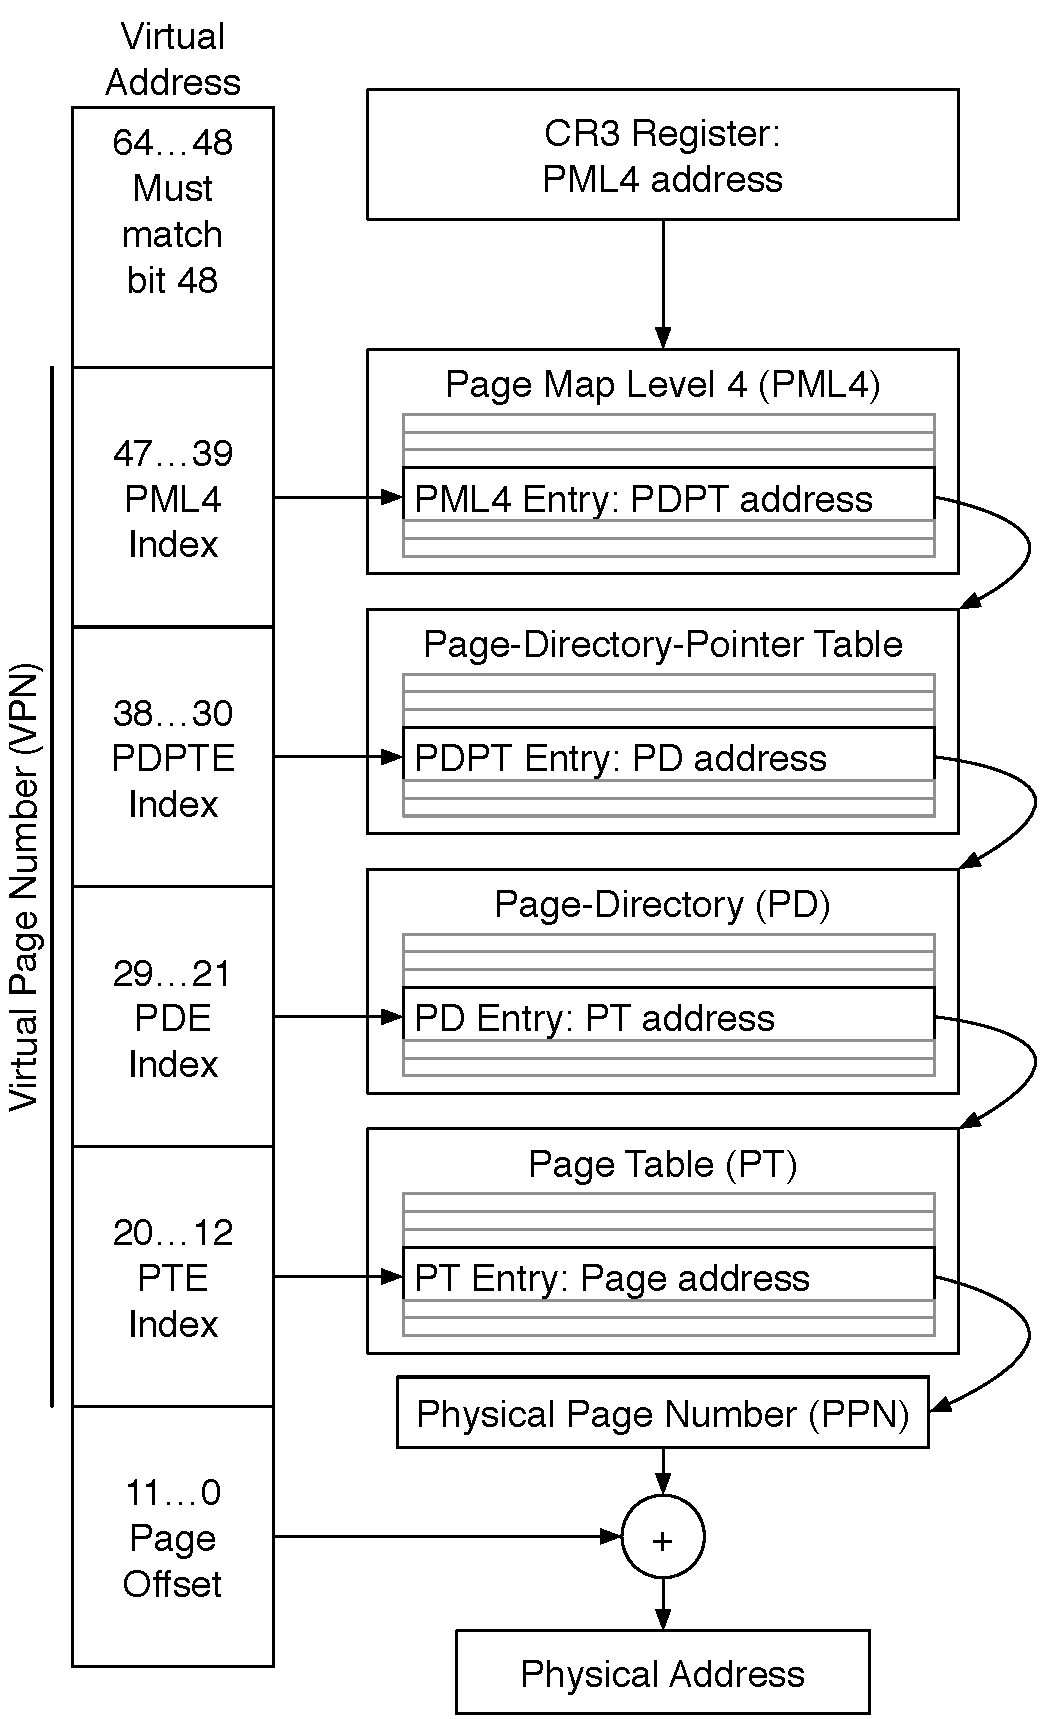
\includegraphics[width=85mm]{figures/os_paging.pdf}}
  \caption{
    IA-32e address translation takes in a 48-bit virtual address and outputs
    a 52-bit physical address.
  }
  \label{fig:os_paging}
\end{figure}

Hypervisors have access to another layer of address translation, named
\textit{extended page tables} (EPT), to multiplex the physical memory across
operating systems. When EPT are enabled, the process above is used to translate
from a virtual address into a \textit{guest-physical address}, effectively
giving each OS kernel the illusion that it controls the entire machine's RAM.
The translation from guest-physical addresses to actual physical addresses uses
the same process as above, except the physical address of the root node is
stored in the extended page table pointer (EPTP) field in the VM's control
structure (VMCS). Figure~\ref{fig:vmx_paging} illustrates the address
translation process in the presence of hardware virtualization.

\begin{figure}[hbtp]
  \center{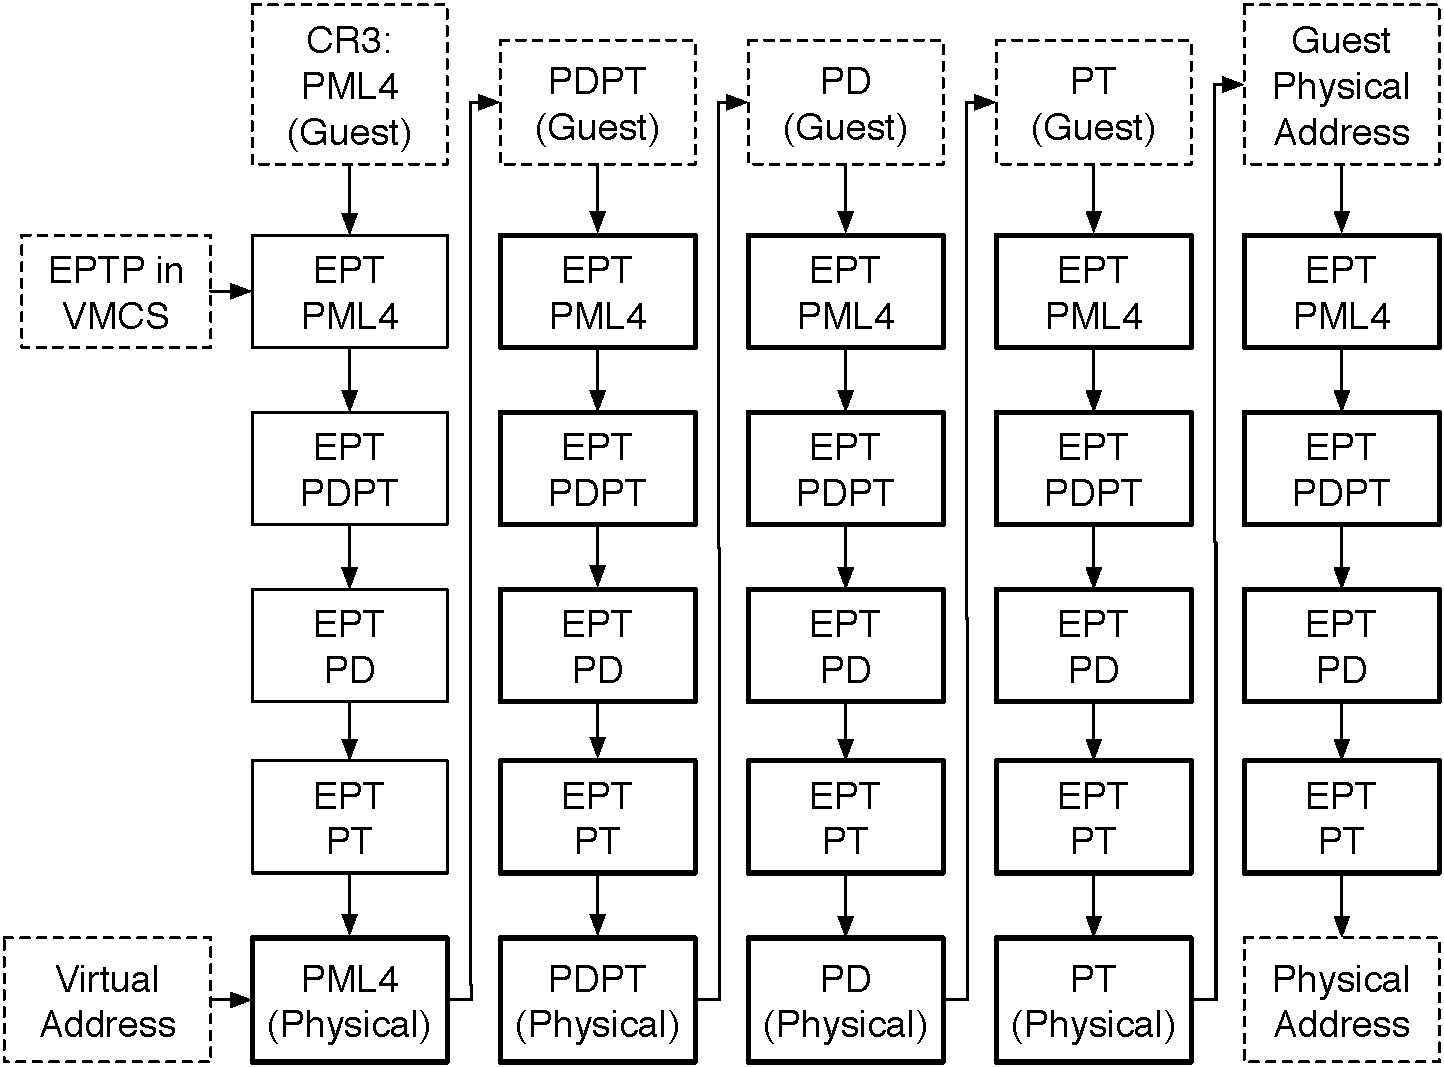
\includegraphics[width=85mm]{figures/vmx_paging.pdf}}
  \caption{
    Address translation when hardware virtualization is enabled. The
    kernel-managed page tables contain guest-physical addresses, so each level
    in the kernel's page table requires a full walk of the hypervisor's
    extended page table (EPT).  A translation requires up to 20 memory accesses
    (the bold boxes), assuming the physical address of the kernel's PML4 is
    cached.
  }
  \label{fig:vmx_paging}
\end{figure}

Each entry in the page tables has some boolean flags, in addition to the
pointer to the next level. The following flags are particularly interesting for
our goals. The \textit{present} (P) flag is set to 0 to indicate pages that
have been evicted from RAM to a cheaper and slower storage medium. When address
translation encounters a page table entry where P is 0, the CPU generates a
page fault (\#PF), and the OS kernel is responsible for loading the page back
into RAM and resuming execution. If an EPT entry has the P flag set to 0, the
CPU performs a VM exit, and the hypervisor has an opportunity to bring the page
into RAM. The \textit{accessed} (A) flag is set to 1 by the CPU whenever the
address translation machinery reads a page table entry, and the \textit{dirty}
(D) flag is set to 1 by the CPU when an entry is accessed by a memory write
operation. The A and D flags give the hypervisor and kernel insight into
application memory access patterns, providing the input for the algorithms that
select which pages get to be evicted from RAM.

Page table entries have flags that provide access control, in addition to the
flags supporting page swapping. The interesting flags are the \textit{writable}
(W) flag, which can be set to 0 to prohibit\footnote{Writes to non-writable
pages result in general protection faults (\#GP).} memory writes to a page, and
the \textit{disable execution} (XD) flag, which can be set to 1 to prevent
instruction fetches from a page.


\subsection{Context Switching}
\label{sec:registers}

Application software targeting the 64-bit Intel architecture uses a variety of
registers to interact with the CPU features. The values in these registers
make up an application's state, or context. Kernels multiplex a CPU among
multiple software threads by \textit{context switching}, namely saving a
thread's context, and replacing it with another thread's previously saved
context. This section covers the context switching features used by SGX when a
logical processor starts or stops executing code that belongs to an enclave.

\begin{figure}[hbt]
  \center{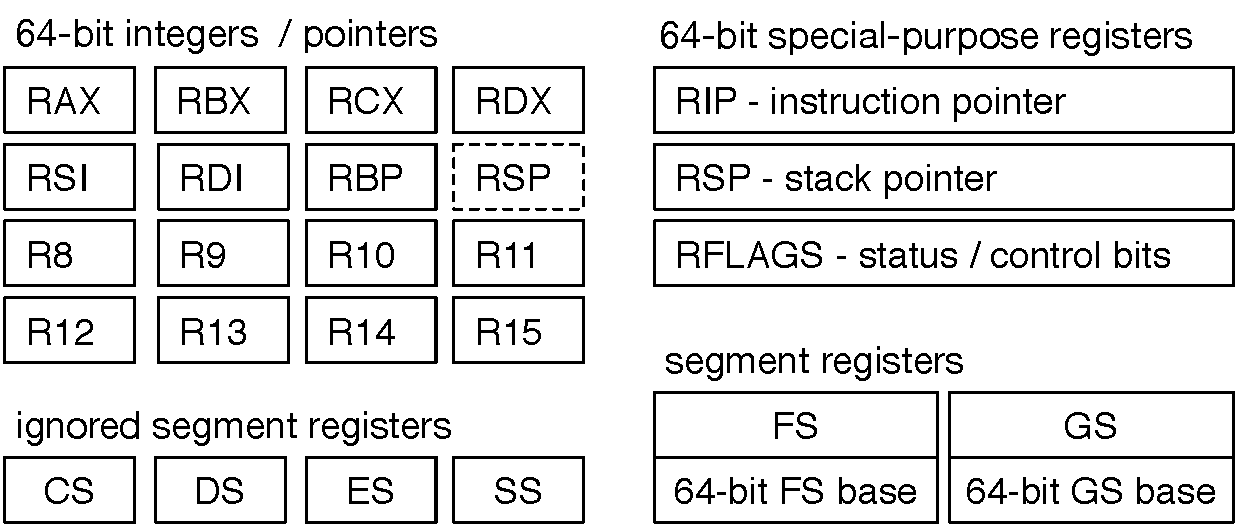
\includegraphics[width=85mm]{figures/cpu_registers.pdf}}
  \caption{
    CPU registers in the 64-bit Intel architecture. RSP can be used as a
    general-purpose register (GPR), e.g., in pointer arithmetic, but it always
    points to the top of the program's stack.
  }
  \label{fig:cpu_registers}
\end{figure}

Integers and memory addresses are stored in 16 \textit{general-purpose
registers} (GPRs). RAX, RBX, RCX, RDX, RSI, RDI, RSP, and RBP are extended
versions of the GPRs available to 32-bit programs, and R9-R16 are new
registers. RSP is reserved for pointing to the top of the \textit{stack}, which
is used to save state during procedure calls.

In 64-bit mode, the values of most segment registers (CS, DS, ES, SS) are
ignored. The FS and GS segment registers generally point to the current
thread's \textit{thread-local storage}, so they are still partially supported
in 64-bit mode. The base addresses loaded in FS and GS are used when computing
linear addresses, whereas the limits are ignored.

All applications also use the RIP register, which contains the address of the
currently executing instruction, and the RFLAGS register, whose bits (e.g.,
the carry flag - CF) are individually used to store comparison results and
control various instructions.

Software might use other registers to interact with specific features, some of
which are shown in Table~\ref{fig:xsave_state}.

\begin{table}[hbt]
  \center{\begin{tabularx}{\columnwidth}{| l | X | l |}
  \hline
  \textbf{Feature} & \textbf{Registers} & \textbf{Feature bit}\\
  \hline
  FPU & FP0 - FP7, FSW, FTW & 0 \\
  \hline
  SSE & MM0 - MM7, XMM0 - XMM15, XMCSR & 1 \\
  \hline
  AVX & YMM0 - YMM15 & 2 \\
  \hline
  \end{tabularx}}
  \caption{Sample feature-specific Intel architecture registers.}
  \label{fig:xsave_state}
\end{table}

The Intel architecture provides a future-proof method for an OS kernel to save
the values of feature-specific registers used by an application. The XSAVE
instruction takes in a bitmap of features, and writes the registers used by
the features whose bits are set to 1 in a memory area that can be used by the
XRESTORE instruction to load the saved values back into feature-specific
registers.

Application software declares the features that it plans to use to the kernel,
so the kernel knows what XSAVE bitmap to use when context-switching. When
receiving the system call, the kernel sets the XCR0 register to the feature
bitmap declared by the application. The CPU generates a fault if application
software attempts to use features that are not enabled by XCR0, so applications
cannot modify feature-specific registers that the kernel wouldn't take into
account when context-switching. The kernel can use the CPUID instruction to
learn the size of the XSAVE memory area for a given feature bitmap, and compute
how much memory it needs to allocate for the context of each of the
application's threads.


\subsection{A Computer Map}

This section maps out a computer using the Intel architecture at three zoom
levels: the motherboard, the CPU, and the execution core, focusing on the
concepts needed to understand SGX and analyze its security properties. Most
details in here are documented in Intel's
\textit{Optimization Reference Manual} \cite{intel2014optimization}.

\subsubsection{The Motherboard}
\label{sec:motherboard}

A computer's components are connected by a printed circuit board called a
\textit{motherboard}, which consists of \textit{sockets} connected by
\textit{buses}. Sockets connect chip-carrying \textit{packages}, to the board.
The Intel documentation uses the term ``package'' to specifically refer to a
CPU.

The buses most relevant to SGX (see Figure~\ref{fig:motherboard} are the
\textit{Quick-Path Interconnect} (QPI) \cite{intel2009qpi}, a network of
point-to-point links that connect processors, the \textit{double data rate}
(DDR) bus that connects a CPU to DRAM, and the \textit{Peripheral Component
Interconnect Express} (PCIe) bus that connects a CPU to peripherals such as a
\textit{Network Interface Card} (NIC).

\begin{figure}[hbt]
  \center{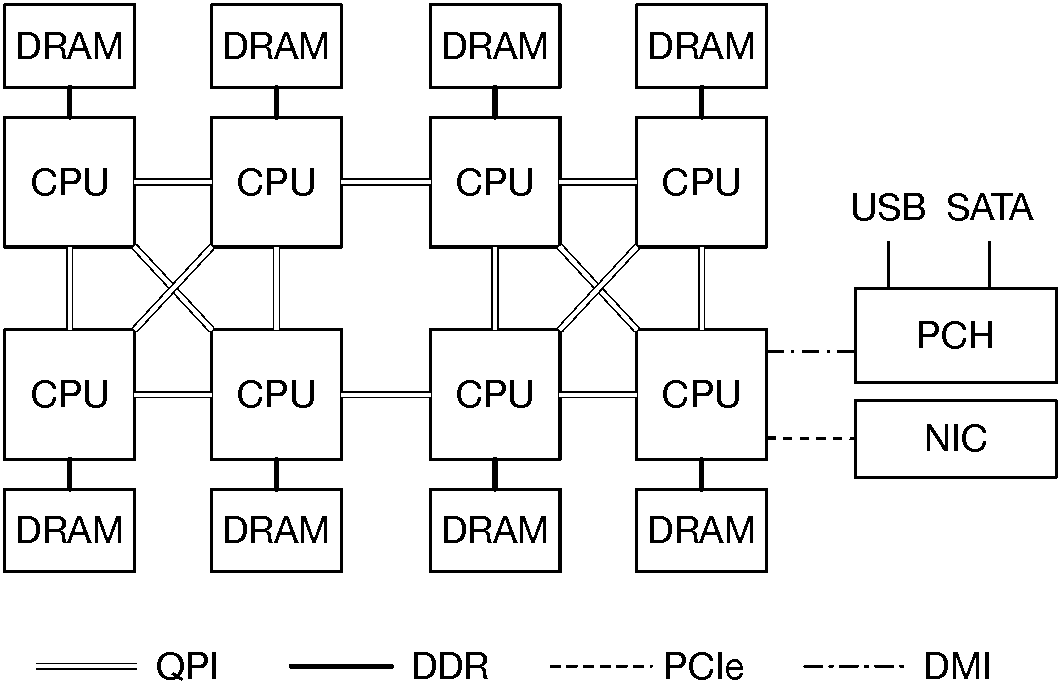
\includegraphics[width=45mm]{figures/motherboard.pdf}}
  \caption{
    The motherboard structures that are most relevant to SGX.
  }
  \label{fig:motherboard}
\end{figure}

The SGX trusted computing base includes the processor package, and excludes the
other hardware in the computer. This implies that, SGX must be able to fend off
attacks from rogue devices, such as the PCIe NIC used to compromise Intel TXT
\cite{wojtczuk2011txt}, as well as passive or active bus-tapping attacks, such
as the memory bus tap used to hack the Xbox \cite{huang2003xbox} and the
memory glitching attack that subverted the PlayStation 3 hypervisor
\cite{hotz2010ps3}.

\subsubsection{The Processor}
\label{sec:cpu_die}

An Intel processor's die, illustrated in Figure~\ref{fig:cpu_die}, is divided
into two broad areas: the \textit{core area} implements the functionality that
comes to mind when thinking of a CPU, while the \textit{uncore} provides
functions that were typically hosted on separate chips, but were integrated to
save power and improve latency.

\begin{figure}[hbt]
  \center{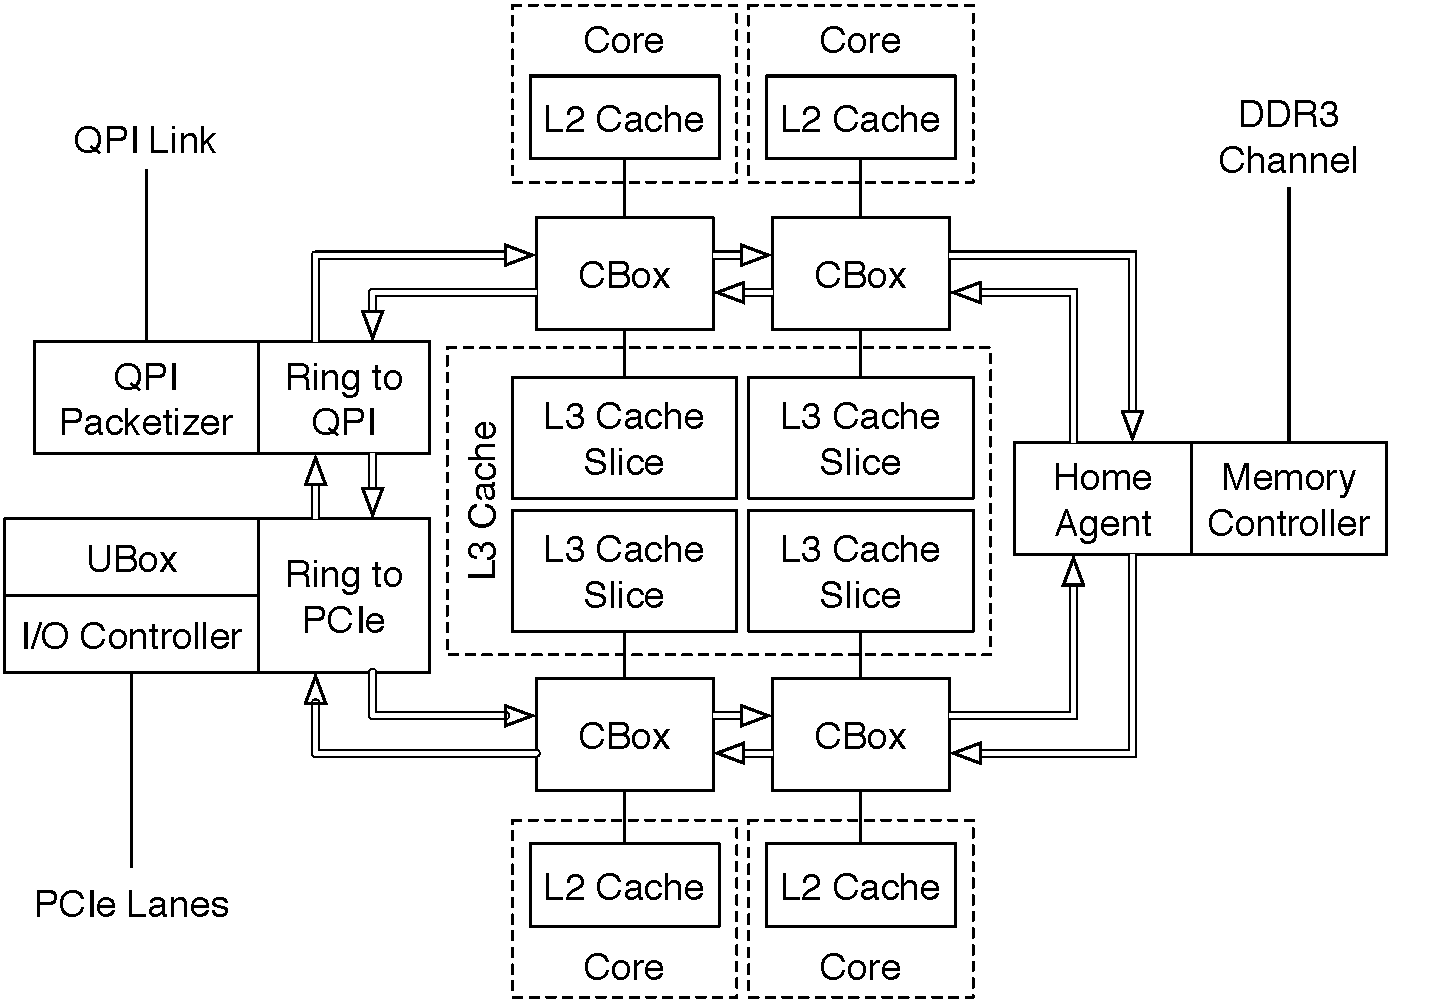
\includegraphics[width=85mm]{figures/cpu_die.pdf}}
  \caption{
    The major components in a modern CPU die. \S~\ref{sec:cpu_die} gives
    an uncore overview. \S~\ref{sec:cpu_core} describes execution cores.
    \S~\ref{sec:cpu_uncore} takes a deeper look at the uncore.
  }
  \label{fig:cpu_die}
\end{figure}

At a conceptual level, the uncore of modern processors includes a memory
controller that interfaces with the DDR bus, an I/O controller that can
arbitrate the PCIe bus, and a growing number of integrated controllers for
peripherals, such as a NIC and a GPU.

The SGX design relies on the fact that the processor die includes the memory
and I/O controller, and thus can prevent any device from accessing protected
memory areas via \textit{Direct Memory Access} (DMA) transfers.
\S~\ref{sec:cpu_uncore} takes a deeper look at the uncore organization and at
the mechanism used by the SGX implementation to protect sensitive memory.

\subsubsection{The Core}
\label{sec:cpu_core}

Virtually all modern Intel processors have core areas consisting of multiple
copies of the execution core circuitry, each of which is called a
\textit{core}.  At the time of this writing, desktop-class Intel CPUs have 4
cores, and server-class CPUs have as many as 18 cores.

Most Intel CPUs feature \textit{hyper-threading}, which means that a core
(shown in Figure~\ref{fig:cpu_core}) has two copies of the register files
backing the execution context described in \S~\ref{sec:registers}, and can
execute two separate streams of instructions simultaneously. Hyper-threading
increases the utilization of the shared fetch, decode and execution units, in
the presence of memory stalls.

\begin{figure}[hbt]
  \center{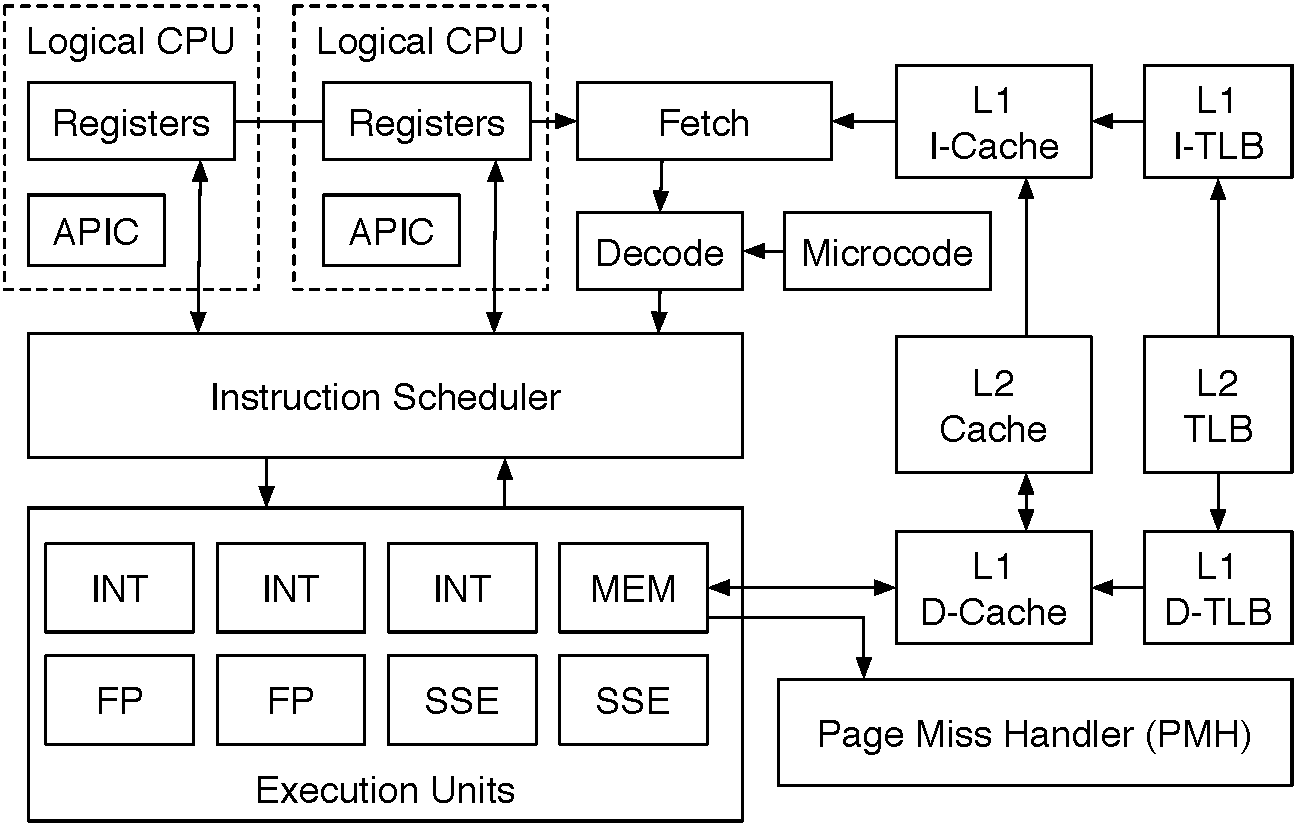
\includegraphics[width=85mm]{figures/cpu_core.pdf}}
  \caption{
    CPU core with two logical processors. Each logical processor has its own
    execution context and local APIC, and they share all the other core
    resources.
  }
  \label{fig:cpu_core}
\end{figure}

A hyper-threaded core is exposed to system software as two \textit{logical
processors}, also named \textit{hardware threads} in the Intel documentation.
The logical processor abstraction allows the code used to distribute work
across processors in a multi-processor system to function without any change on
multi-core hyper-threaded processors.

The high level of resource sharing introduced by hyper-threading introduces a
security vulnerability. Software running on one logical processor can use the
high-performance counter \cite{petters1999making} to get information about the
instructions and memory access patterns of another piece of software that is
executed on the other logical processor in the same core.


\subsection{CPU Microcode}
\label{sec:microcode}

Intel's SGX patents disclose that all the SGX features, except for DRAM
encryption, were implemented as microcode extensions. This section explains the
microcode feature in Intel CPUs. The limitations of microcode can explain
seemingly arbitrary decisions in the SGX design, and a thorough understanding
is crucial to evaluating the feasibility of SGX modification proposals.

The x86 architecture defines a \textit{complex instruction set} (CISC).
However, virtually all modern CPUs are architected following \textit{reduced
instruction set} (RISC) principles. This is accomplished by having the
instruction decode stage (see Figure~\ref{fig:cpu_core}) break down each x86
instruction into \textit{micro-ops} for every instruction. The other CPU stages
work exclusively with micro-ops.

The majority of x86 instructions are handled by the hardware decoding path,
which can emit at most 4 micro-ops per instruction. Complex instructions use a
slower decoding path that reads micro-ops from a \textit{microcode store ROM}
(MSROM).

Modern Intel processors implement a microcode update facility. The SDM
describes microcode updates from the perspective of an OS kernel and
hypervisor. Each core can be updated independently, and the updates must be
re-applied on each boot cycle. A core can be updated multiple times, but each
update must have a bigger version than the core's current version.

The update facility increases the attractiveness of developing architectural
features as microcode extensions. The SGX enclave measurements produced by the
processor include the microcode version, hinting that the SGX designers
anticipated the need to use microcode updates.

\cite{hawkes2012microcode} used fault injection and timing analysis to conclude
that each recent Intel microcode update is signed with a 2048-bit RSA key and
a (possibly non-standard) 256-bit hash algorithm. This implies that Intel
already has a microcode implementation of RSA-2048 signature checking, which
may explain why SGX uses RSA signatures in its enclave structures.

\cite{chen2014microcode} sets out to analyze the structure of microcode used in
all x86 processors, but is unable to obtain any details about Intel's
microcode. Fortunately, even though the microcode structure is undocumented,
the 4 micro-ops limitation can be used to guess intelligently whether an
architectural feature is implemented in microcode. For example, the context
switch in \S~\ref{sec:registers} is most likely done in microcode, whereas
simple arithmetic and memory access is handled directly by hardware.


\subsection{Memory Caching}
\label{sec:caching}

Caches are small, fast memories that store recently accessed code and data.
Thanks to the high locality in the memory access patterns of most applications,
good caches have very high hit rates (90\%-99\%), and do a great job of hiding
the (comparatively) high latency of DRAM. At the same time, the large time
differences between cached and un-cached memory accesses can be used to learn
about an application's memory access patterns, via
\textit{cache timing attacks} \cite{banescu2011cache}. The patterns, in turn,
can reveal private information, such as whether certain bits in an encryption
key are set or not.

This section describes the caching concepts needed to understand our claim that
cache timing attacks can be used to obtain fine-grained memory access patterns
for the software running inside an SGX enclave. \cite{smith1982cache},
\cite{patterson2013architecture} and \cite{hennessy2012architecture} all
provide good backgrounds on low-level cache implementation concepts.

Desktop-class Intel CPUs have three levels of cache memory. Each core has its
own L1 and L2, and all cores share an L3 cache. This means that a cache timing
attack that aims at the L2 cache would have to rely on the hypervisor or kernel
to schedule a hardware thread on a logical processor in the same core as the
target software, whereas an attack on the L3 cache can be performed using any
logical processor on the same CPU.

The \textit{cache line} is the atomic unit of data transfer between the caches
and the main memory. The cache line size is always a power of two. Assuming
$n$-bit memory addresses and a cache line size of $2^{l}$ bytes, the lowest
$l$ bits of a memory address are an offset into a cache line, and the highest
$n - l$ bits determine the cache line that is used to store the data at the
memory location. All recent processors have 64-byte cache lines.

The L1 and L2 caches in recent processors are multi-way set-associative with
direct set indexing, as shown in Figure~\ref{fig:cpu_cache}. A $W$-way
set-associative cache has its memory divided into \textit{sets}, where each set
has $W$ lines. A memory location can be cached in any of the $w$ lines in a
specific set that is determined by the highest $n - l$ bits of the location's
memory address. Direct set indexing means that the $S$ sets in a cache are
indexed from $0$ to $S - 1$, and a memory location is cached in the set with
index $address_{n - 1 \ldots n - l} \bmod S$. In the common case where the
number of sets in a cache is a power of two, so $S = 2^{s}$, the lowest $l$
bits in an address make up the cache line offset, the next $s$ bits are the set
index. The highest $n - s - l$ bits in an address are not used when selecting
where a memory location will be cached. Figure~\ref{fig:cpu_cache} shows the
cache structure and lookup process.

\begin{figure}[hbt]
  \center{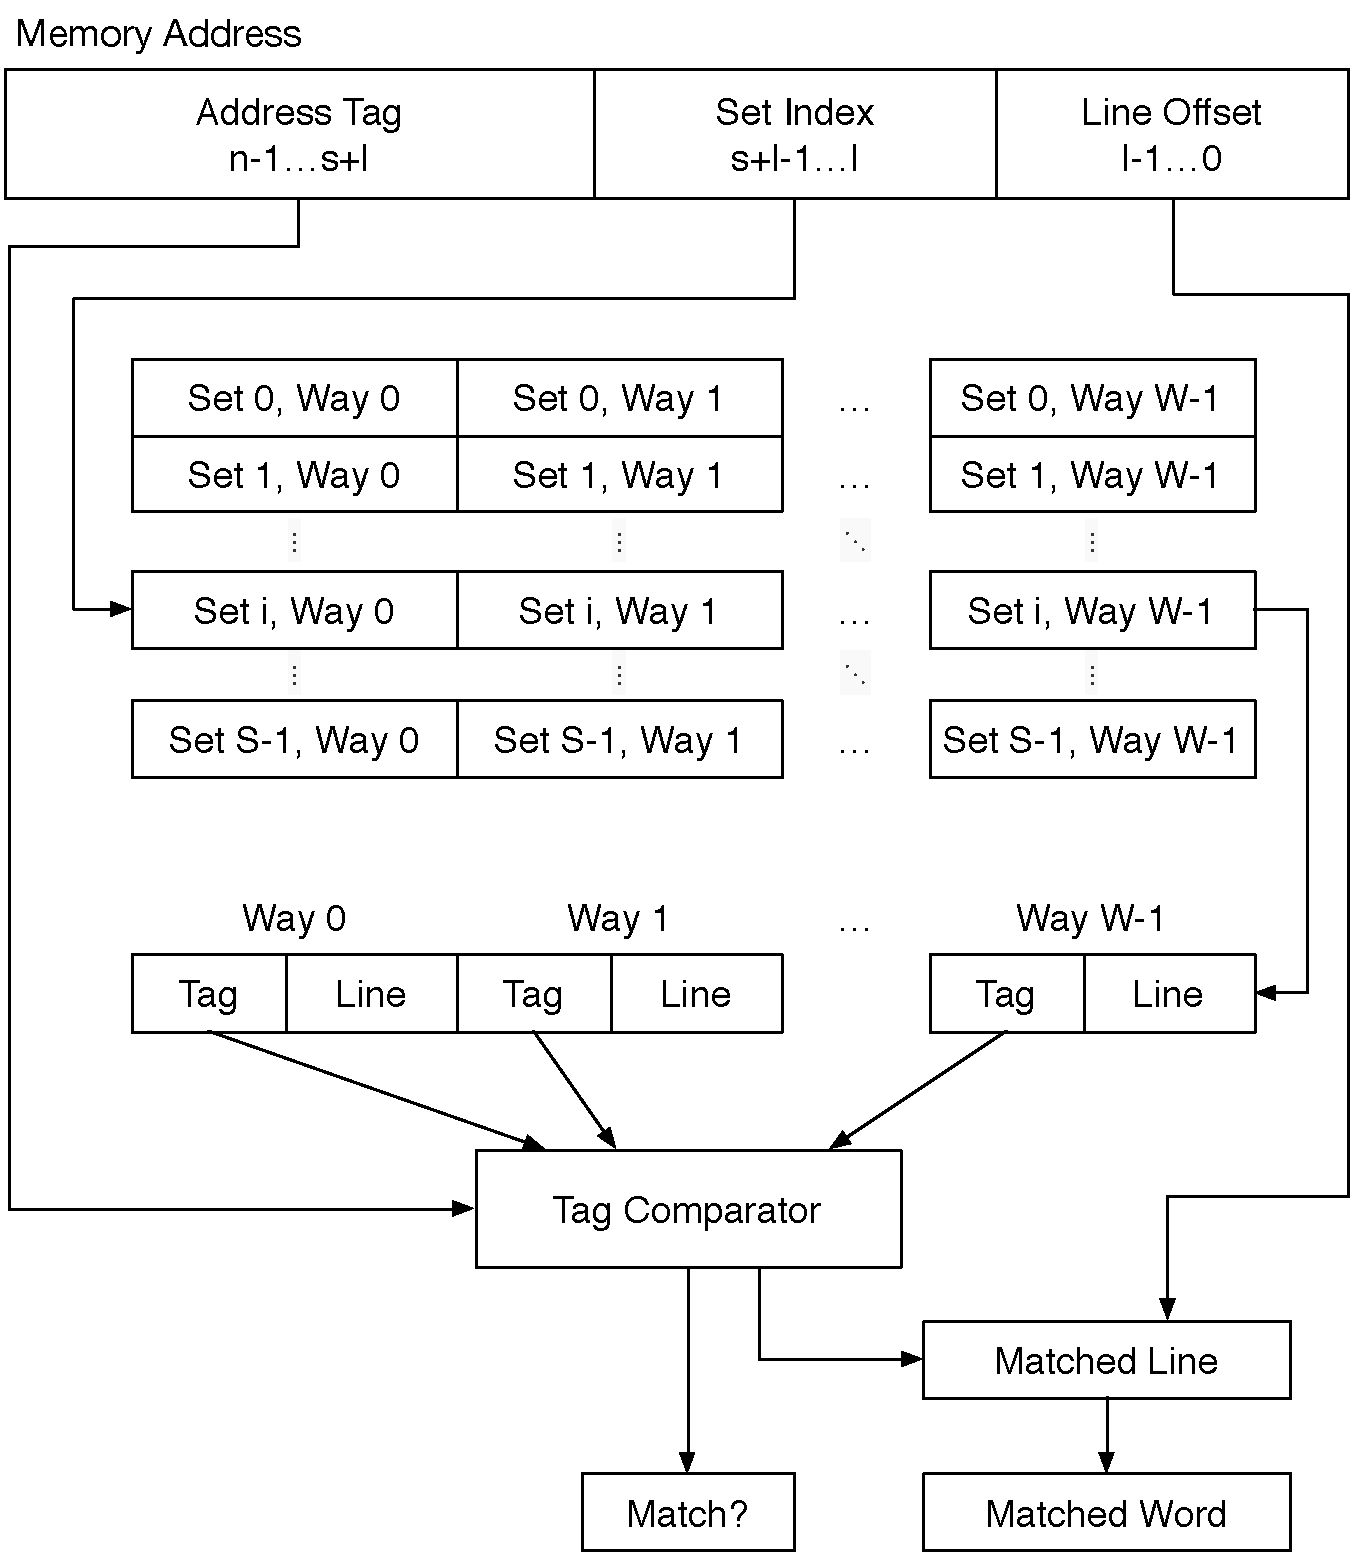
\includegraphics[width=85mm]{figures/cpu_cache.pdf}}
  \caption{
    Cache organization and lookup, for a $W$-way set-associative cache with
    $2^{l}$-byte lines and $S = 2^{s}$ sets. The cache works with $n$-bit
    memory addresses. The lowest $l$ address bits point to a specific byte in a
    cache line, the next $s$ bytes index the set, and the highest $n - s - l$
    bits are used to decide if the desired address is in one of the $W$ lines
    in the indexed set.
  }
  \label{fig:cpu_cache}
\end{figure}

The SDM does not describe the L3 indexing scheme, but we develop some
understanding of it in \S~\ref{sec:cpu_uncore}.


\subsection{Caching and Address Translation}
\label{sec:tlbs}

Address translation (described in \S~\ref{sec:paging}) requires up to 4 memory
accesses for a 64-bit bare-metal kernel, and up to 16 memory accesses when a
hypervisor is present. To achieve high clock speeds, the CPU caches address
translations in \textit{translation look-aside buffers} (TLBs).

The set index in an L1 cache only uses the address bits that are not impacted
by address translation, so that set lookup and TLB lookup can be done in
parallel. Given a page size $P = 2^{p}$ bytes, the requirement above is
equivalent to $l + s \le p$. In the x86 architecture $p = 12$, and all recent
processors have 64-byte cache lines ($l = 6$) and 64 sets ($s = 6$), as shown
in Figure~\ref{fig:caching_and_paging}.

\begin{figure}[hbt]
  \center{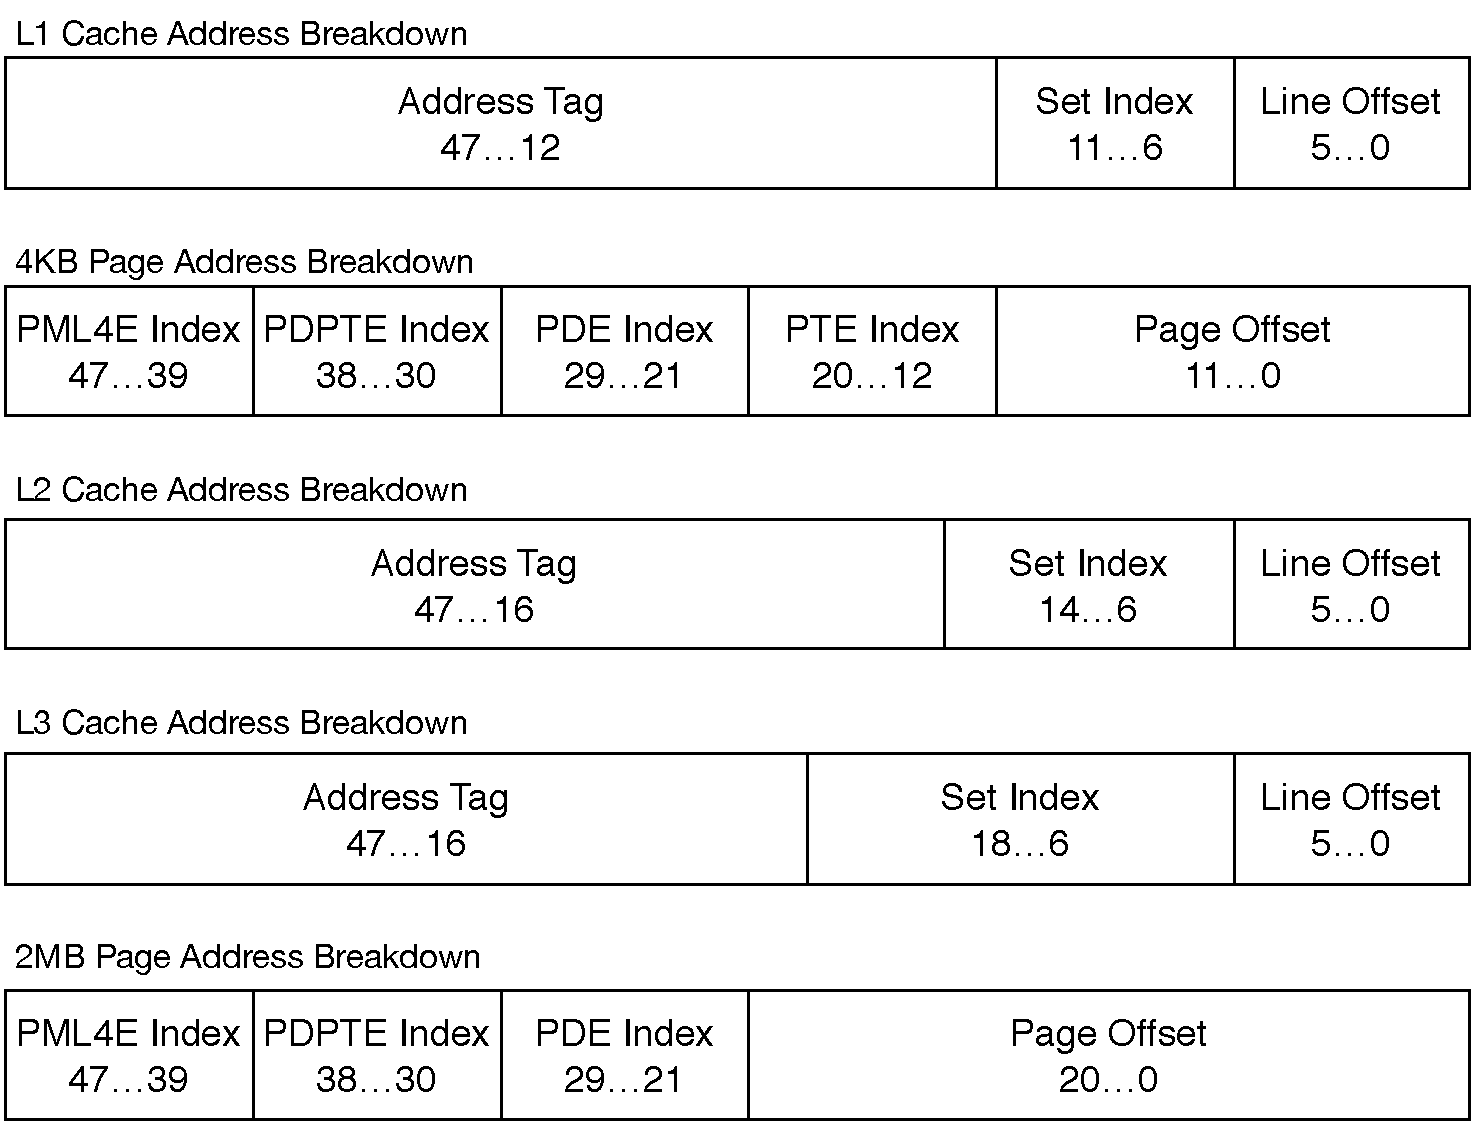
\includegraphics[width=85mm]{figures/caching_and_paging.pdf}}
  \caption{
    Virtual addresses from the perspective of cache lookup and address
    translation. The bits used for the L1 set index and line offset are not
    changed by address translation, so the page tables do not impact L1 cache
    placement. Page tables do impact L2 and L3 cache placement. Using large
    pages (2MB or 1GB) makes cache placement independent of page tables.
  }
  \label{fig:caching_and_paging}
\end{figure}

The L2 cache in recent Intel processors uses physical indexing
\cite{patterson2013architecture}. The indexing method is not documented in
Intel's manuals and is not reported by the CPUID instruction, as it is
considered to be an implementation detail. However, the indexing method
determines the set index for a given memory location, and knowing which memory
addresses are stored in the same set is crucial for mounting and defending
against cache timing attacks.

\begin{figure}[hbt]
  \center{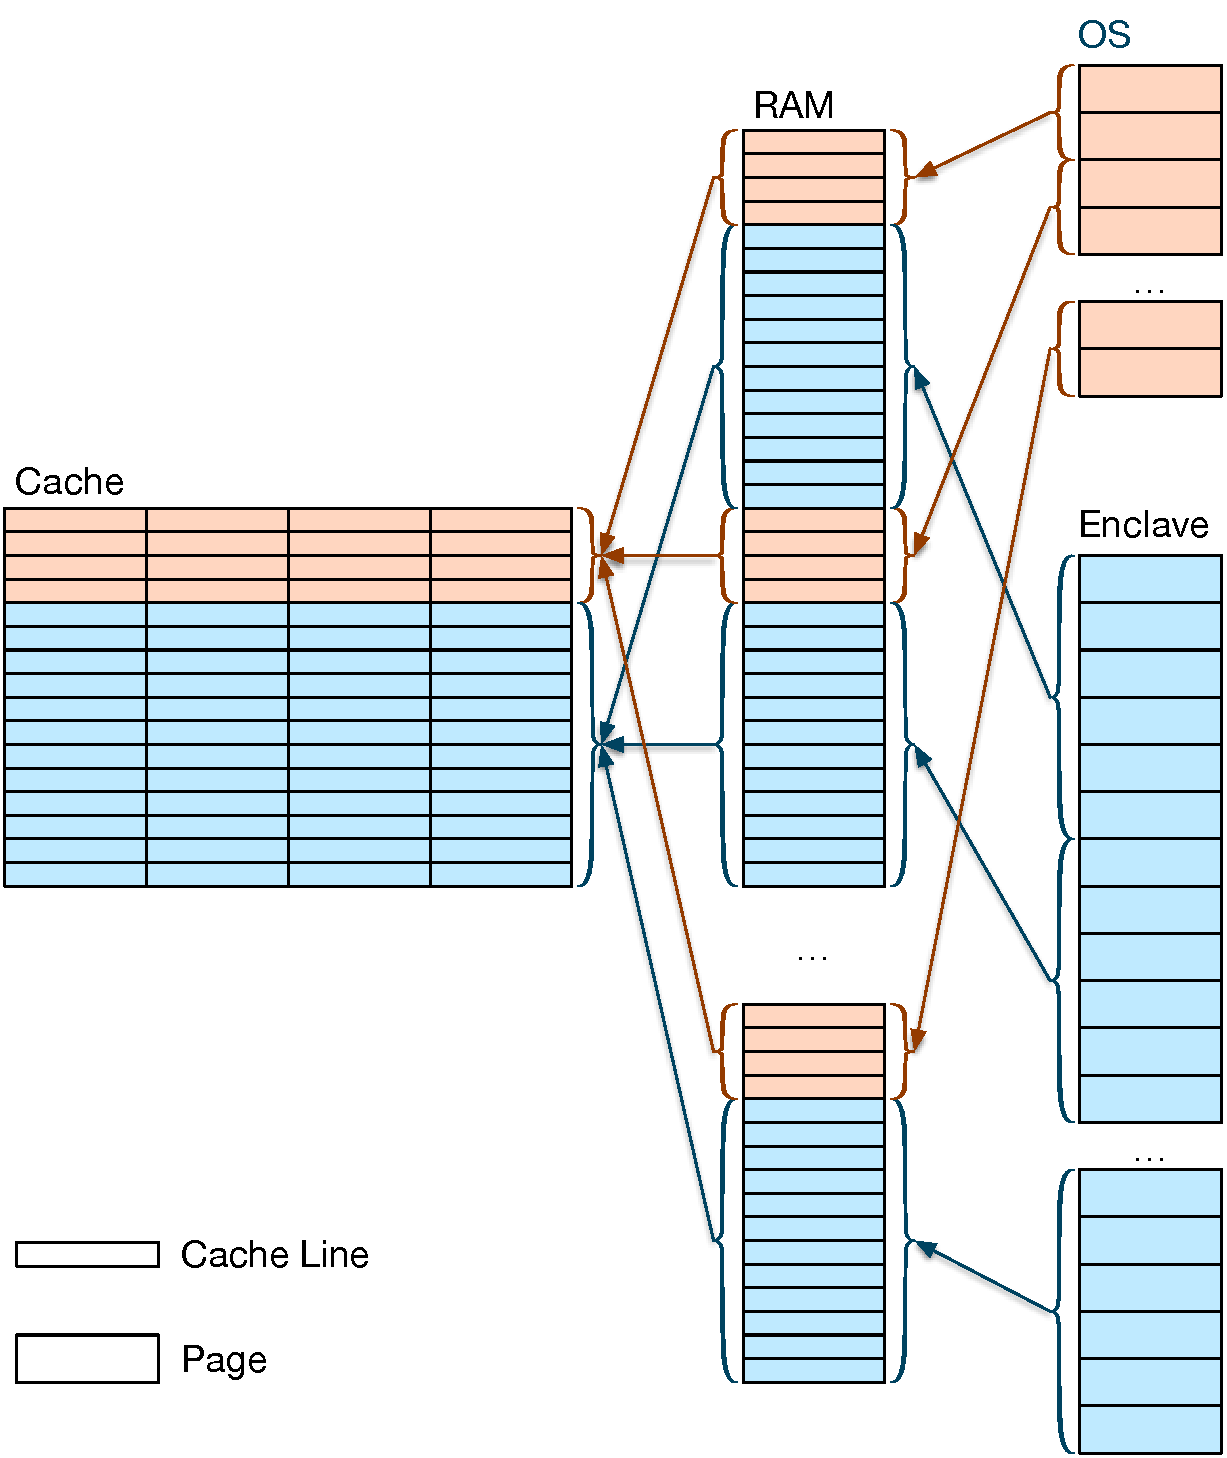
\includegraphics[width=85mm]{figures/cache_partitions.pdf}}
  \caption{
    Cache partitioning between two applications. Each application has some
    cache sets allocated to it, and only uses RAM regions that map to its cache
    sets. When partitioning the L1 cache, applications have to follow this
    constraint themselves. When the L2 cache is partitioned, the OS can map the
    pages in an application's virtual address space to the RAM regions that the
    application can use, so applications are oblivious to the cache
    partitioning.
  }
  \label{fig:cache_partitions}
\end{figure}

The system software is responsible for invalidating TLBs when it changes the
page tables that it manages. The Intel architecture has instructions that can
be used by the kernel and hypervisor to invalidate the TLB entries covering a
specific linear address. Some instructions invalidate all the TLB entries as a
side-effect.


\subsection{Caching and Logical Processors}
\label{sec:cache_coherence}

Intel's SDM describes the ordering guarantees that a software developer can
rely on when accessing the same memory location in multiple hardware threads.
The memory model is a variation on the Total Store Order (TSO) model
\cite{owens2009tso}, meaning that all the hardware threads will see the same
order of writes.

When the hardware threads that access the same memory location execute on
different cores, they may cause the cache line containing the memory location
to be loaded in each core's L1 and L2 cache. In order to provide TSO guarantees
in these circumstances, the processor cores use a \textit{cache coherence
protocol} that keeps the cache line copies in sync.

% Propagation of Paging-Structure Changes to Multiple Processors: SDM S 4.10.5

The cache coherence does not cover TLB entries. When modifying a page table
or EPT, the kernel and hypervisor are responsible for performing a
\textit{TLB shootdown}, which consists of stopping all the logical processors
that use the page table / EPT about to be changed, performing the changes,
executing TLB-invalidating instructions on the stopped logical processors, and
then resuming execution on the stopped logical processors.

\cite{hennessy2012architecture} provides a good introduction to cache coherence
principles. Intel's optimization reference \cite{intel2014optimization} states
that the coherence protocol used in Intel processors is
MESIF \cite{goodman2009mesif}, a variant of MESI.


\subsection{The Memory Subsystem}
\label{sec:cpu_uncore}

According to Intel's patents, the SGX memory protection relies on special
entries in the \textit{Source Address Decoder} (SAD) and \textit{Target Address
Decoder} (TAD).  A thorough understanding of the memory hierarchy is required
in order to understand this aspect of the SGX implementation.

The QPI protocol layer defines the cache coherence protocol, which is a variant
of MESIF \cite{goodman2009mesif}, an extension of MESI. The QPI protocol
defines caching agents, which are connected to the last-level cache in a
processor, and home agents, which are connected to memory controllers. Cache
agents make requests to home agents for cache line data on cache misses, while
home agents keep track of cache line ownership, and obtain the cache line data
from other cache line agents, or from the memory controller. Each processor has
its own home agent and caching agents.

On recent Intel processors, most of the memory hierarchy is implemented on the
processor chip. The Intel documentation refers to these on-chip components as
\textit{the uncore}. The uncore structure is described in some processor
family datasheets \cite{intel2014datasheet,intel2010datasheet}, and in the
overview sections in Intel's uncore performance monitoring documentation
\cite{intel2014uncore, intel2012uncore, intel2010uncore}.

UBox - uncore configuration controller; master for reading and writing
physically distributed registers across the uncore using the message
channel; receives interrupts from system and dispatches them to the
appropriate core; system lock master (e.g. QPI bus lock)

CBox - last-level cache (LLC) coherence engine; the interface between a core
and a slice of the LLC; acts as the QPI cache agent for that slice of LLC;
CBoxes are co-located with cores and connected in a ring interconnect

The physical memory space is split up between CBoxes. The ``complex'' caching
algorithm mentioned in the Intel SDM includes a ``hashing'' step that maps a
physical address to a CBox, and thus a slice of the LLC.

Each CBox contains a Source Address Decoder (SAD), and the configurations of
all SADs in a core are identical, replicated by the UBox. The SAD takes in a
memory address and access type, and outputs a transaction type (coherent,
non-coherent, IO) and a node ID.

Home agent - contains the Target Address Decoder (TAD) and interfaces with a
memory controller; a CPU may contain multiple home agents, if it has multiple
memory contollers; the TAD maps a memory address to a specific DRAM channel,
implements logical channel address mapping and interleaving;


\section{Data Structures}
\label{sec:enclaves}

The central context of SGX is the \textit{enclave}, a protected environment
that contains the code and data pertaining to a security-sensitive computation.
This section provides an overview of the data structures used by an enclave.


\subsection{Enclaves and the RAM}

% PRM: SGX S 3.5

The enclaves' code and data is stored in \textit{Processor Reserved Memory}
(PRM), a contiguous range of RAM that cannot be directly accessed by other
software, including privileged software such as the SMM code, the hypervisor,
and the OS kernel. The CPU also prevents devices attached to the system bus
from performing DMA transfers to/from the PRM. This is possible because, on
modern systems, the northbridge is integrated into the CPU
(see Figure \ref{fig:pch}).

On systems with SGX-enabled CPUs, the BIOS is responsible for setting aside a
contiguous range of RAM for \textit{Processor Reserved Memory} (PRM). The
CPU prevents most programs (including the SMM handler, the hypervisor and the
operating system kernel) from accessing the PRM.


The PRM must be set up to use SGX features and, once configured, the PRM range
cannot be changed. Furthermore, the PRM's size must be an integer power of two,
and its start address must be aligned to the same power of two. The range
restrictions reduce the complexity of checking if a RAM address is in the PRM
to a bitwise AND and an equality comparison.

\begin{figure}[hbtp]
  \center{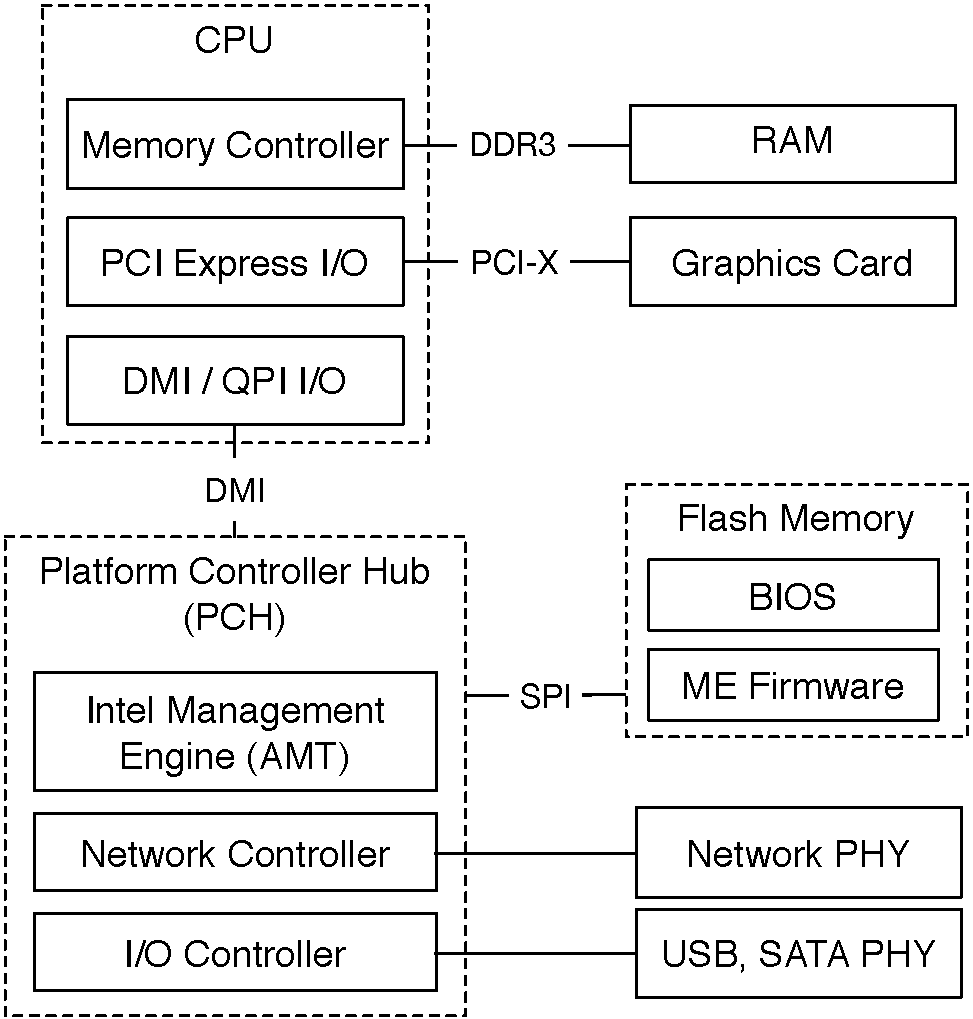
\includegraphics[width=65mm]{figures/pch.pdf}}
  \caption{
    The architecture of modern Intel systems.
    The Platform Controller Hub (PCH) contains a service processor, called the
    Intel Management Engine (ME). The processor has direct access to the
    network, can read and modify RAM via DMA transfers, and can override the
    CPU boot vector. The processor runs firmware stored in the same flash
    memory as the BIOS code.
  }
  \label{fig:pch}
\end{figure}

% EPC and EPCM: SGX S 1.5, S 1.5.1, S 2.6.13, S 3.5, S 3.5.1

The contents of enclaves and the associated data structures are stored in the
\textit{Enclave Page Cache} (EPC). The EPC is a subset of the PRM

, so the
protection measures described in the paragraphs above ensure that the enclaves'
memory cannot be read or tampered with by any malicious software running on the
host computer, or by malicious peripherals attached to the system bus. The
stringent restrictions placed on PRM documented above reduce the probability of
bugs in the security checks at the foundation for SGX's integrity and privacy
guarantees.

The EPC is split into 4kb pages, which are allocated to enclaves or supporting
data structures by the \textit{system software}, which can be either a
\textit{hypervisor} (the software running in VMX root mode at ring 0), or a
\textit{kernel} (the code inside an operating system running at ring 0).

The CPU maintains some metadata for each EPC page into the \textit{Enclave Page
Cache Map} (EPCM), which is used to ensure that an enclave does not attempt to
access another enclave's pages, and that system software manages EPC pages in a
way that is consistent with the SGX security model. The SGX documentation does
not state where the EPCM is stored, but we can hypothesize that it is either
an on-chip memory, like the L3 cache, or stored in a PRM region that is not
used by the EPC.

% SECINFO: SGX S 2.6.5, S 2.6.5.{1,2}

\subsection{Enclave Structures}

Each enclave has a \textit{SGX Enclave Control Structure} (SECS)


% SECS: SGX S 2.6.1, S 2.6.1.1,


% TCS: SGX S 2.6.2, S 2.6.2.{1,2,3,4}


% SSA: SGX S 2.6.3,

\section{Security Model}
\label{sec:attestation}

THe central context of SGX is the \textit{enclave}, a protected environment
that contains the code and data pertaining to a security-sensitive computation.
An SGX-enabled processor protects the integrity and privacy of the computation
inside an enclave by isolating the enclave's code and data from the outside
environment, including the operating system and hypervisor, and hardware
devices attached to the system bus. At the same time, the SGX model remains
compatible with the the traditional software layering in the Intel
architecture, where the OS kernel and hypervisor manage the computer's
resources. The rest of this section describes the security properties of
enclaves, discussing the trade-offs made while trying to balance security with
backwards compatibility.



Enclaves were designed to contain and protect the privacy-sensitive parts of an
application. All the code that handles private data must receive integrity
protection. Otherwise, a hostile environment could modify the code to leak
information about private data. Therefore, the SGX programming model prescribes
that code which accesses private data must be entirely contained inside an
enclave. Jumping into and out of enclave code must be performed explicitly
using the dedicated instructions \texttt{EENTER} and \texttt{EEXIT}.

The code inside an enclave runs at ring 3 (user mode), so it has the same
privileges as regular application code (see Figure \ref{fig:cpu_rings}).

\begin{figure}[hbtp]
  \center{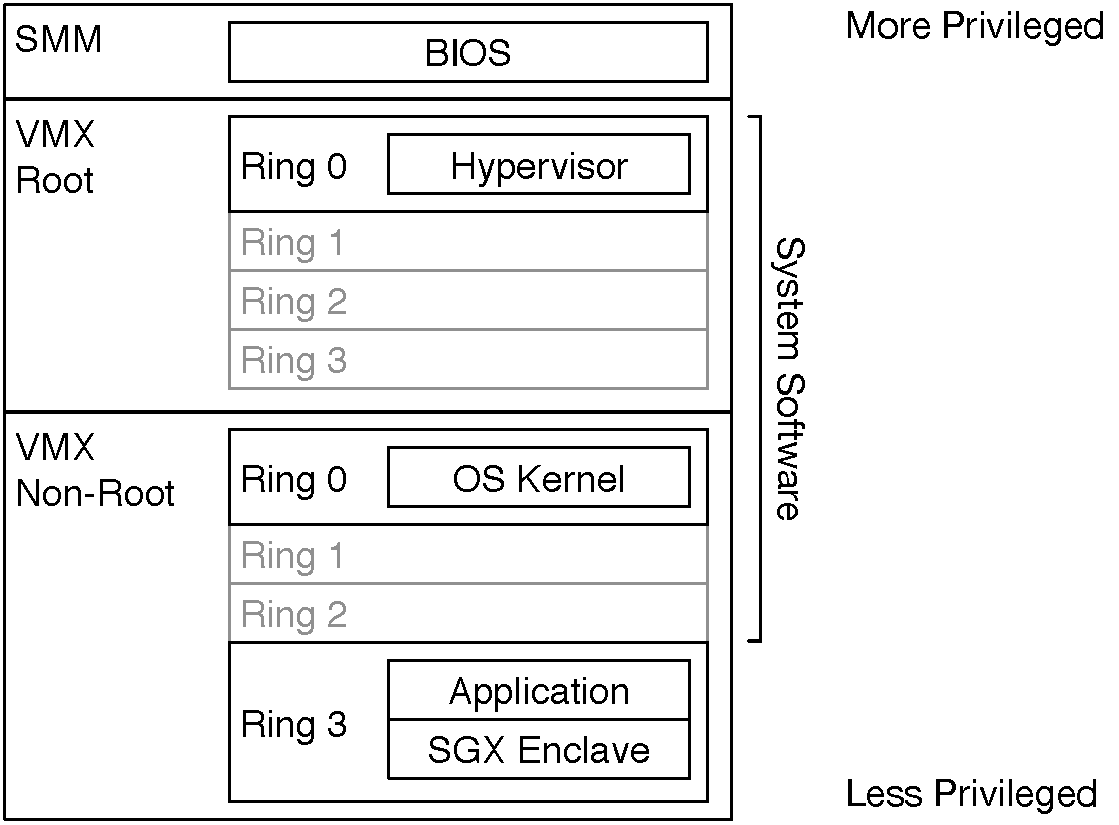
\includegraphics[width=75mm]{figures/cpu_rings.pdf}}
  \caption{
    Enclaves hold an application's private data and the code that operates on
    it. Therefore, they run at ring 3, in user mode.
  }
  \label{fig:computing_model}
\end{figure}

%\section{Software Guard Extensions (SGX)}
\label{sec:sgx}

This section summarizes the aspects of the SGX documentation that are relevant
to our system. The interested but time-constrained reader is advised to read
\cite{mckeen2013innovative}, \cite{anati2013sgx}, and Chapters 1 (Introduction
to SGX), 3 (Enclave Operation), 4 (Enclave Exiting Events) and 6 (SGX
Interactions with IA32 and Intel 64 Architecture) of \cite{intel2013sgxmanual}
for a deeper understanding of SGX.


\subsection{SGX Overview}
\label{sec:sgx_overview}

SGX introduces a protected execution environment, called an \textit{enclave}.
An enclave's code and data are protected by placing them inside the Enclave
Page Cache (EPC), which is a subset of the Processor Reserved Memory (PRM)
area. The EPC is split in 4KB pages. Each page is associated with an enclave.
EPC page memory accesses coming from code outside the EPC page's enclave are
blocked by the CPU. This access check covers all privilege levels, including
SMM. The memory controller inside the CPU blocks any DMA access to PRM, so EPC
pages cannot be accessed by hardware via DMA.

The EPC contents is encrypted\footnote{Actually, the SGX manual carefully
tiptoes around this issue by saying ``On implementations in which EPC is part
of system DRAM, the contents of the EPC are protected by an encryption
engine.''} as it leaves the CPU, to prevent against bus tapping attacks.
Although the data is encrypted, the memory addresses are not protected,
exposing the enclave code's memory access patterns.

Execution flow can only enter an enclave via special CPU instructions
(\texttt{EENTER}, \texttt{ERESUME}, \texttt{EEXIT}), which are similar to the
mechanism for switching from user mode to kernel mode. Enclave execution always
happens in protected mode, at ring 3, and uses the address translation set up
by the OS kernel and hypervisor (\S \ref{sec:paging}). \texttt{EENTER}
transfers control to a predefined entry point in the enclave, and
\texttt{EEXIT} leaves the enclave.

To avoid leaking private data, a CPU that is executing enclave code does not
directly service an interrupt, fault (e.g., a page fault) or VM exit. Instead,
the CPU first performs an Asynchronous Enclave Exit (AEX) to switch from
enclave code to ring 3 code, and then services the interrupt, fault, or VM
exit.  The CPU performs an AEX by saving the CPU state into a predefined area
inside the enclave and transfers control to a pre-specified instruction outside
the enclave, replacing CPU registers with synthetic values. After the
interrupt, fault or VM exit is serviced, its handler returns control to ring 3
code outside the enclave, which performs an \texttt{ERESUME}, which transfers
control back into the enclave and restores the CPU state at the time the
enclave execution was interrupted.

The allocation of EPC pages to enclaves is delegated to the OS kernel (or
hypervisor), and done via dedicated ring 0 CPU instructions. \texttt{EADD}
allocates new pages to an enclave under construction, and \texttt{EREMOVE}
deallocates pages during enclave tear-down. \texttt{EWB} evicts\footnote{
Multi-threaded enclaves require more steps that are orthogonal to the issues
addressed by this work.} an EPC page to RAM space that the OS kernel can
access, and \texttt{ELDB}\footnote{SGX specifies two related instructions,
\texttt{ELDB} and \texttt{ELDU}. The distinction is irrelevant for our
purposes.} loads a previously evicted page from kernel-acessible RAM back into
the EPC.

\texttt{EADD} associates each EPC page with a virtual address used to access
it, and the association is maintained by the \texttt{EWB} / \texttt{ELDB} pair.
The CPU enforces\footnote{The CPU generates a general protection fault (\#GP)
if an address translation that results in an EPC page uses the wrong virtual
address as input.} the invariant that an EPC page can only be accessed using
the virtual address associated with it. This mechanism ensures that the OS
kernel and hypervisor maintain a consistent mapping of virtual addresses to
EPC pages. The CPU encrypts and HMACs pages evicted with \texttt{EWB},
providing privacy and integrity guarantees, including protection against replay
attacks. The details are described in \cite{intel2013sgxmanual}.

Page faults in enclave code are handled using the AEX process. The CR2
register, which normally holds the virtual address that causes the fault, has
its bottom 12 bits set to zero. The other bits of CR2 are necessary for the OS
kernel or hypervisor to know which page needs to be loaded in RAM or into the
EPC. This allows a curious OS kernel or hypervisor to obtain a page-level
memory access trace for a program running inside an enclave, simply by making
sure that only one page is present at any given time.


\subsection{SGX Information Leaks}
\label{sec:sgx_leaks}

Software Guard Extensions, as documented in \cite{intel2013sgxmanual}, does not
provide full privacy guarantees to the code executing inside an enclave. We
present methods that an attacker can use to extract information from an
enclave.

\subsubsection{Hyper-Threading Leaks}

Modern Intel CPUs feature hyper-threading, which means that each core has two
(or more) sets of register files and local APICs, presented as logical
processors running separate threads (see Figure \ref{fig:cpu_core}). The
threads share the other core resources, such as the fetch and decode units,
execution units and L1 and L2 caches. SGX does not prevent hyper-threading, so
a malicious OS kernel or hypervisor can schedule a thread executing enclave
code and a snooping thread on logical processors on same core. The snooping
thread can use the processor's high-resolution performance counter
\cite{petters1999making} to get information about the instructions and memory
access patterns of the thread executing enclave code.

A promising approach for preventing against hyper-threading leaks is to
effectively disable hyper-threading, by using \texttt{CPUID} to find out the
number of logical processors in the current core, and to require the OS to
schedule threads in the same enclave on all the logical processors. This could
be implemented by having the main thread spinlock waiting for the other threads
to start, before any protected computation is performed. However, a malicious
kernel or hypervisor can de-schedule the other threads after the main thread
performed the spinlock check, so this defense is not reliable.

\subsubsection{Page-Level Memory Access Leaks}

While executing the code inside an enclave, the CPU still follows the standard
page translation process (\S \ref{sec:paging}), including setting the A and D
bits and delivering page faults. A malicious OS kernel or hypervisor can
obtain the page-level trace of an application executing inside an enclave by
setting the P flag to 0 on all the enclave's pages before starting enclave
execution, and then maintaining exactly one instruction page and one data page
present in the enclave's address space.

When a page fault is generated, CR2 contains the virtual address of a page
accessed by enclave, and the error code indicates whether the memory access was
a read or a write (bit 1) and whether the memory access is a data access or
an instruction fetch access (bit 4). On a data access, the kernel tracing the
enclave code's memory access pattern would set the P flag of the desired page
to 1, and set the P flag of the previously accessed data page to 0. Instruction
accesses can be handled in a similar manner.

For a slightly more detailed trace, the kernel can set a desired page's W flag
to 0 if the page fault's error code indicates a read access, and only set it to
1 for write accesses. Also, applications that use a page as both code and data
(self-modifying code and just-in-time compiling VMs) can be handled by setting
a page's XD flag to 0 for a data access, and by carefully accounting for the
case where the last accessed data page is the same as the last accessed code
page.

Leaving an enclave via an AEX and re-entering the enclave via \texttt{ERESUME}
causes the CPU to flush TLB entries that contain enclave addresses, so a
tracing kernel would not need to worry about flushing the TLB. The tracing
kernel does not need to flush the caches either, because the CPU needs to
perform address translation even for cached data.

An easy way to reduce this attack's power is to increase the page size, so the
trace contains less information. However, the attack cannot be completely
prevented without removing the kernel's ability to oversubscribe the EPC,
which is a major benefit of paging.

\subsubsection{Fine-Grained Memory Access Leaks}

The AEX process and the \texttt{ERESUME} instructions do not flush the CPU
caches. A tracing kernel can take advantage of cache timing to narrow down
the addresses in an application's memory access trace to cache line
granularity, by extending the method described above with the steps below.

The tracing kernel controls the mapping between virtual addresses and physical
addresses, so it can make sure that its own code and data use different sets
in the L2 cache from the enclave's code and data. For example, in a typical
256kb (per-core) L2 cache organized as 512 8-way sets of 64-byte lines, the
tracing kernel could allocate lines 0-63 for the enclave's code page, lines
64-127 for the enclave's data page, and use lines 128-511 for its own pages.

Right before entering an enclave via \texttt{EENTER} or \texttt{ERESUME}, the
kernel would issue \texttt{CLFLUSH} instructions to flush the enclave's code
page and data page from the cache. The enclave could have accessed a single
code page and a single data page, so flushing the cache should be reasonably
efficient. The tracing kernel then uses 16 bogus pages (8 for the enclave's
code page, and 8 for the enclave's data page) to load all the 8 ways in the 128
cache sets allocated by enclave pages. After an AEX gives control back to the
tracing kernel, it can read the 16 bogus pages, and exploit the time difference
between an L2 cache hit and a miss to see which cache lines were evicted and
replaced by the enclave's memory accesses.

\subsubsection{Leaks via Physical Attacks}

The methods described above rely on a compromised hypervisor or OS kernel, but
not on physical attacks. If an attacker can tap into the memory bus and read
the address lines, the attacker can learn the enclave code's memory access
patterns, at a fine granularity.

The processor reserved memory (PRM) is configured by the BIOS at boot time as
a continuous memory area, and can be configured as write-back (WB) or
uncacheable (UC) memory. If the PRM is uncacheable, the CPU will generate a
memory transaction for every memory access. The granularity of the memory
transactions depends on the encryption engine used for the EPC, which is not
documented in \cite{intel2013sgxmanual}. If 128-bit AES is used, memory tapping
would yield addresses at 16-byte granularity, which means two 64-bit words.

At the same time, configuring the PRM as uncacheable memory removes the cache
timing attack documented above, at the cost of dramatically slowing down the
execution of SGX code. In this case, the CPU would still leak memory access
patterns at page granularity, due to the address translation engine.

%\input{contents/fixes.tex}

\setlength{\bibsep}{1pt}
\small
\bibliographystyle{plain}
%\bibliographystyle{abbrv}
\bibliography{references}

\end{document}
